\chapter{Project Development}\label{ch:project-development}

This chapter provides an in-depth look into the development of Chronocademy, outlining the key aspects that contributed to its creation.
The following sections will cover essential areas of the project, including product development, user experience, developer experience, the technologies used, and the code architecture.

Each of these areas played a critical role in shaping Chronocademy into a functional and user-friendly platform.
From defining the product's core features and refining its usability to selecting the right tools and structuring the codebase, this chapter highlights the processes and decisions that guided the project from concept to development.

By exploring these topics, the reader will gain a comprehensive understanding of how the team approached the challenges of building Chronocademy and the methods they used to ensure a robust, scalable, and well-designed platform.


\section{Product Development}\label{sec:productdevelopment}
The development of Chronocademy began by defining, refining, and prioritizing its core aspects and features.
This section outlines the step-by-step process undertaken to shape the product, ensuring it was both viable and aligned with the needs of its users.

\subsection{Defining the Idea through the Business Model Canvas}\label{subsec:business-model-canvas}
The first step in the product development journey was to define the core idea behind Chronocademy.
To structure and validate this concept, the team utilized the Business Model Canvas framework.

\begin{quote}
    ``The Business Model Canvas is a strategic management and entrepreneurial tool.
    It allows you to describe, design, challenge, invent, and pivot your business model.
    This method from the bestselling management book Business Model Generation is applied in leading organizations and start-ups worldwide.''
\end{quote}\cite[Business Canvas Model]{business-canvas-model}

This tool helped identify the key components of the platform, including the value proposition, target customer segments, revenue streams, cost structure, among others.
By analyzing these elements, the team was able to understand how Chronocademy would create, deliver, and capture value in a competitive landscape.
The structured approach of the Business Model Canvas ensured that the idea was not only innovative but also practical and sustainable.

\begin{figure}[h]
    \centering
    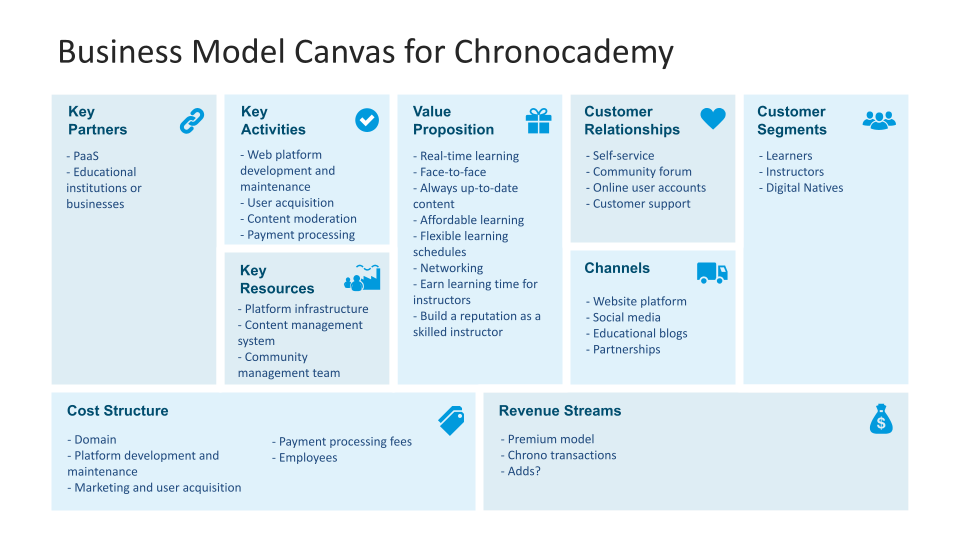
\includegraphics[width=14cm]{business-canvas-model}
    \caption{Business Model Canvas}
    \label{fig:figure1}
\end{figure}

\underline{Key resources:}
\begin{itemize}
    \item Online platform infrastructure: Website development and maintenance for user accounts, course listings, scheduling, and video conferencing.
    \item Content management system (CMS): A system to allow instructors to upload course descriptions and materials.
    \item Community management team: Answer to user requests, ensure a positive learning environment and moderate.
\end{itemize}

\underline{Key activities:}
\begin{itemize}
    \item Web platform development and maintenance: Develop and continuously update and improve the website for optimal user experience.
    \item User acquisition: Marketing strategies to attract users.
    \item Content moderation: Moderate courses to ensure quality.
    \item Payment processing: Implement a secure system for handling transactions.
\end{itemize}

\underline{Key partnerships:}
\begin{itemize}
    \item Video conferencing platform: Integrate a reliable video conferencing service for online lessons.
    \item Educational institutions or businesses.
    \item Payment processing companies: Integrate a secure payment processor.
\end{itemize}

\underline{Value propositions:}
\begin{itemize}
    \item Real-time learning face-to-face: Access to a wide range of skills and knowledge from instructors in real-time face-to-face.
    \item Always up-to-date content.
    \item Affordable learning: Main payment goes through a time-based exchange system.
    \item Flexible learning schedules: Using calendars and through online video conferencing.
    \item Networking: Opportunity to connect with a community of learners and instructors.
    \item Earn learning time for instructors: Then can be used to acquire new skills and knowledge themselves.
    \item Build a reputation as a skilled instructor: Thanks to students feedback and ratings.
\end{itemize}

\underline{Customer relationships:}
\begin{itemize}
    \item Self-service: Learners and instructors can work autonomous.
    \item Community forum: Create a forum for learners and instructors to interact, ask questions, and share experiences.
    \item Online user accounts: Users will create accounts to manage their learning time, browse courses, schedule lessons, and provide feedback.
    \item Customer support: Offer email or chat support for users encountering technical difficulties, needing assistance or providing feedback.
\end{itemize}

\underline{Customer segment:}
\begin{itemize}
    \item Learners: Persons trying to acquire new knowledge through real-time instruction.
    \item Instructors: Persons with expertise willing to share their knowledge and earn learning time.
    \item Digital natives.
\end{itemize}

\underline{Channels:}
\begin{itemize}
    \item Website: Primary channel for user registration, course browsing, lesson scheduling, and video conferencing.
    Centralised platform.
    \item Social media: Used for marketing, promotion, and building a community around Chronocademy.
    \item Educational blogs or partnerships: Collaborate with educational blogs or platforms to promote Chronocademy and reach potential learners.
\end{itemize}

\underline{Cost structure:}
\begin{itemize}
    \item Domain: Pay and maintain the internet domain over time.
    \item Platform development and maintenance: Costs associated with website development, hosting, and ongoing maintenance.
    \item Marketing and user acquisition: Costs for online advertising and social media marketing.
    \item Content moderation: Costs associated with managing the course submission process and ensuring lessons quality.
    \item Payment processing fees: Fees charged by payment processors for handling transactions.
    \item Community management team: Costs associated with management of the online community.
\end{itemize}

\underline{Revenue streams:}
\begin{itemize}
    \item Premium model: It offers free Chrono, access to exclusive lessons scripts and a better advertisement for teachers.
    \item Chrono transactions: Charge for transactions fees either for buying or selling Chronos.
    \item Ads: Include ads (not very intrusive).
\end{itemize}

After completing the Business Model Canvas, the team had a clear understanding of the platform's value proposition, target audience, revenue streams, and cost structure.
This work laid the groundwork for the subsequent stages of product development.

\subsection{Establishing the Brand: Colors, Logo, and Slogans}\label{subsec:colors-logo-slogans}
With the foundation of the business model in place, the second step was establishing a unique and memorable brand identity for Chronocademy.
The team selected a color palette that reflected the platform’s values of knowledge, reliability and accessibility.
The logo was designed to be simple yet distinctive, incorporating elements that represent time spent on learning and growth.
As well as the name, Chronocademy, which combines the words ``chronos'' (latin for time) and ``academy'' to emphasize the platform's focus on real-time learning.
Slogans were thought to be a good match with the platform, such as ``Learn.
Teach.
Grow.'' These branding efforts were crucial for creating a meaningful identity with the target audience and set Chronocademy apart in the market.

\subsubsection{Color Palette}\label{subsubsec:color-palette}
The color palette for Chronocademy was chosen following the colors theory, which is

\begin{quote}
    ``a set of practices for picking colours together for harmonious designs and contextual combinations''
\end{quote}\cite[The Color Theory]{colorTheory}.

The first step was to decide which tone of colors would be used, and the team decided to use some warm colors to give a sense of energy and modern product instead of pastel colors, which are know for their calming and trustworthy interpretation.

Once the color analysis was defined, the team started to work on the style tiles to actually pick the exact colors for the brand.
Style tiles are a design tool defined as:

\begin{quote}
    ``a design deliverable consisting of fonts, colors and interface elements that communicate the essence of a visual brand for the web
    [\ldots]
    They help form a common visual language between the designers and the stakeholders and provide a catalyst for discussions around the preferences and goals of the client.
    [\ldots]
    Style tiles establish a direct connection with actual interface elements without defining layout.''
\end{quote}\cite[Style Tiles]{styleTiles}

The first step to build the style tile board was to define the concept: \textit{``knowledgeable, reliable, and accessible''}.
Then, we searched for images and illustrations that would represent those words and extract the colors out of them.
By doing this a couple of times, we ended up with two different style tiles that were combined to create the final one, by using the fonts of tile number 1 and colors of tile number 2.\newline

\begin{figure}[h]
    \centering
    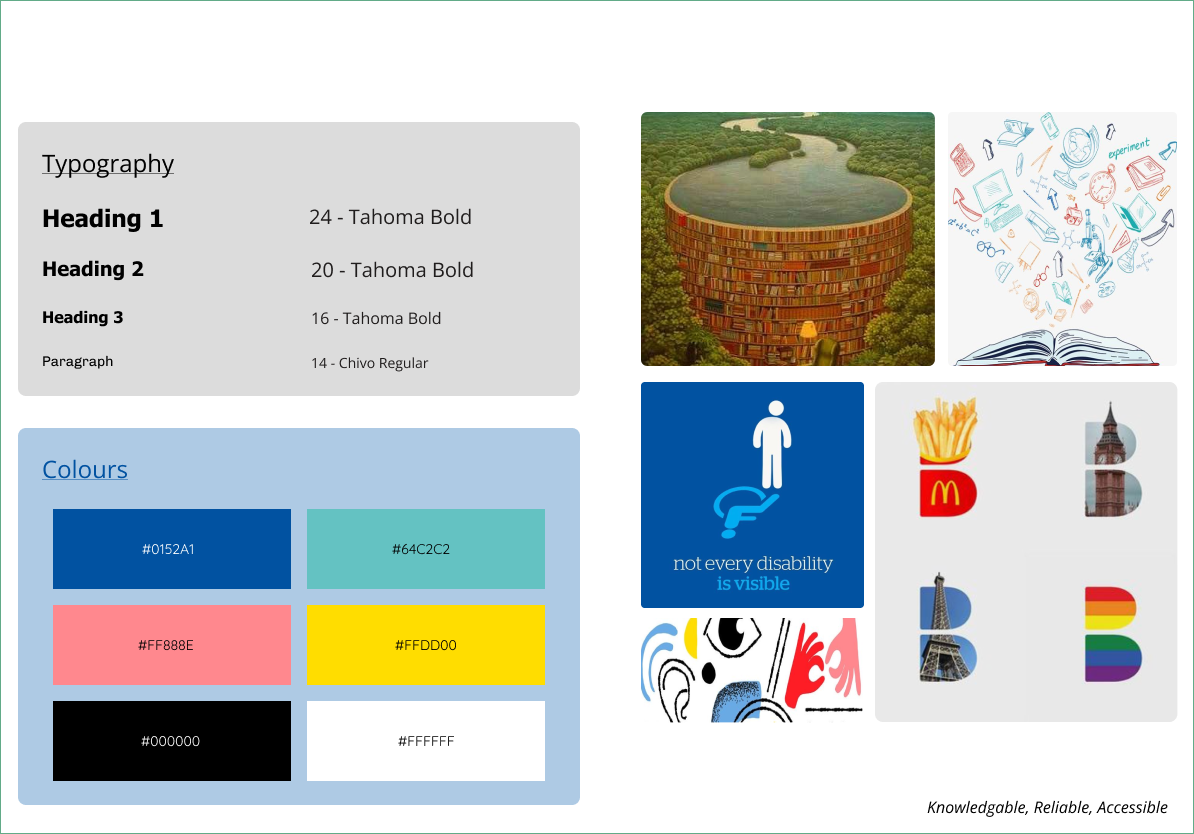
\includegraphics[width=14cm]{style-tile-1}
    \caption{Style Tile 1}
    \label{fig:figure2}
\end{figure}
\begin{figure}[h]
    \centering
    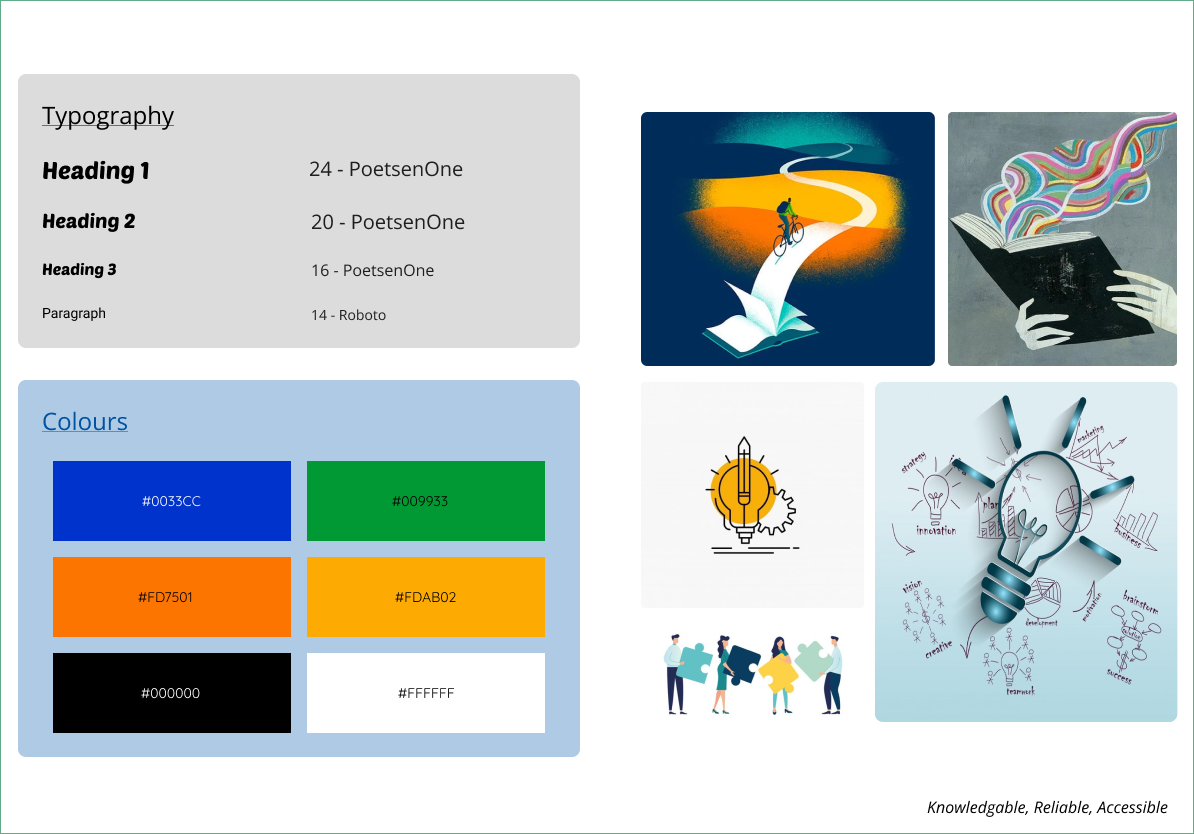
\includegraphics[width=14cm]{style-tile-2}
    \caption{Style Tile 2}
    \centering
    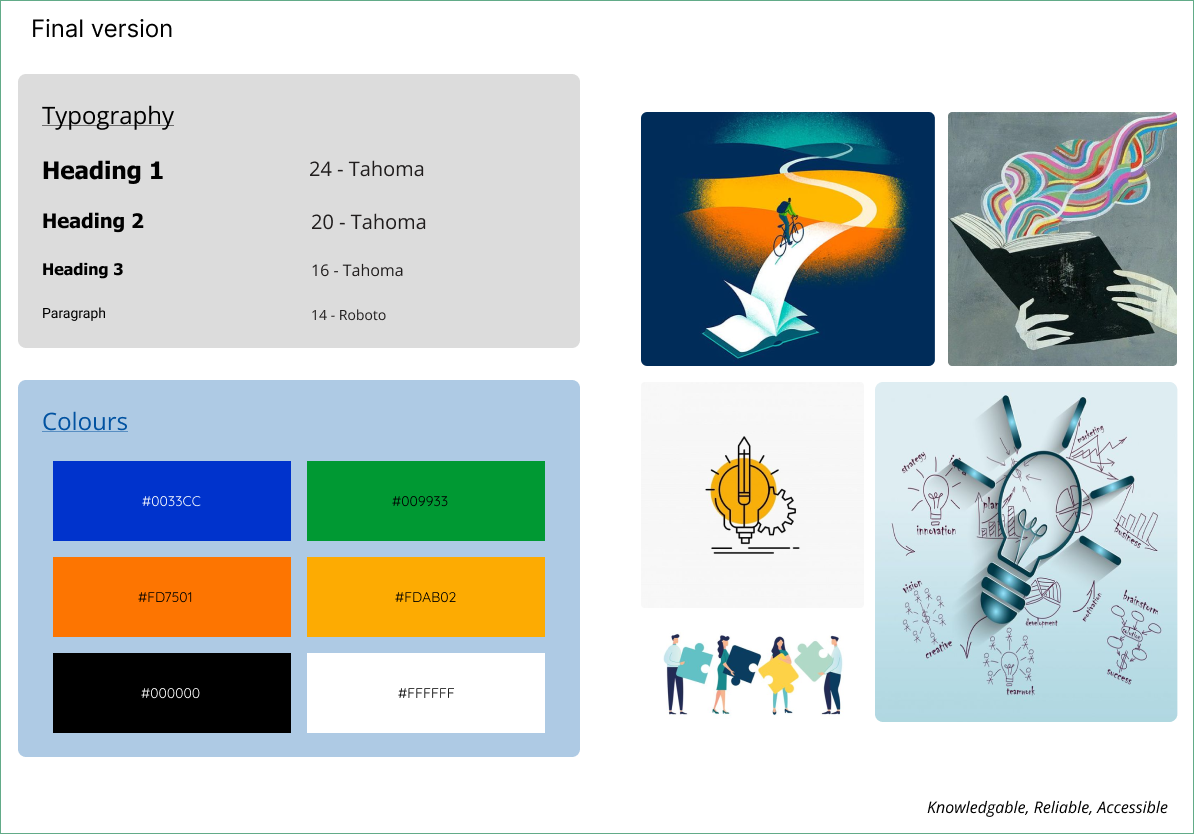
\includegraphics[width=14cm]{style-tile-final}
    \caption{Style Tile Final}
    \label{fig:figure3}
\end{figure}
This tool was helpful to come up with the final color palette and fonts that would be used in the platform.
All three versions were focused on the same concept of \textit{``knowledgeable, reliable, and accessible''}.
\clearpage

\newpage
\subsubsection{Logo}\label{subsubsec:logo}
The Chronocademy logo was designed to visually represent the core themes of the platform—time, learning, and innovation.
The logo features an hourglass shape, symbolizing the platform's unique time-based credit system.
This visual metaphor reflects the idea that time is a valuable currency within the learning experience, emphasizing the platform’s core functionality of exchanging time for knowledge.
The hourglass is split into two distinct sections, reinforcing the concept of time management and the structured nature of the educational experience.

The warm orange hue used in the hourglass conveys energy, creativity, and a welcoming atmosphere.
This vibrant color contrasts with the bold, black typography, creating a modern and professional aesthetic that suggests reliability and sophistication.
The choice of a clean, sans-serif font enhances the logo’s readability and reflects the platform’s user-friendly, technology-driven approach.

The design also subtly emphasizes the two-way interaction between learners and instructors.
Just as sand flows between chambers in an hourglass, knowledge is exchanged between users on the platform.
We wanted the logo to visually encapsulate this idea.

We believe that by combining a recognizable time-based symbol with a clean, contemporary design, the Chronocademy logo effectively communicates the platform's key values, knowledge, accessibility, and reliability.
It serves not only as a brand identifier but also as a visual reminder of the platform’s unique approach to learning through time-based exchanges.

Here the reader can see some of the logo options that were considered before the final decision was made.

\begin{figure}[h]
    \centering
    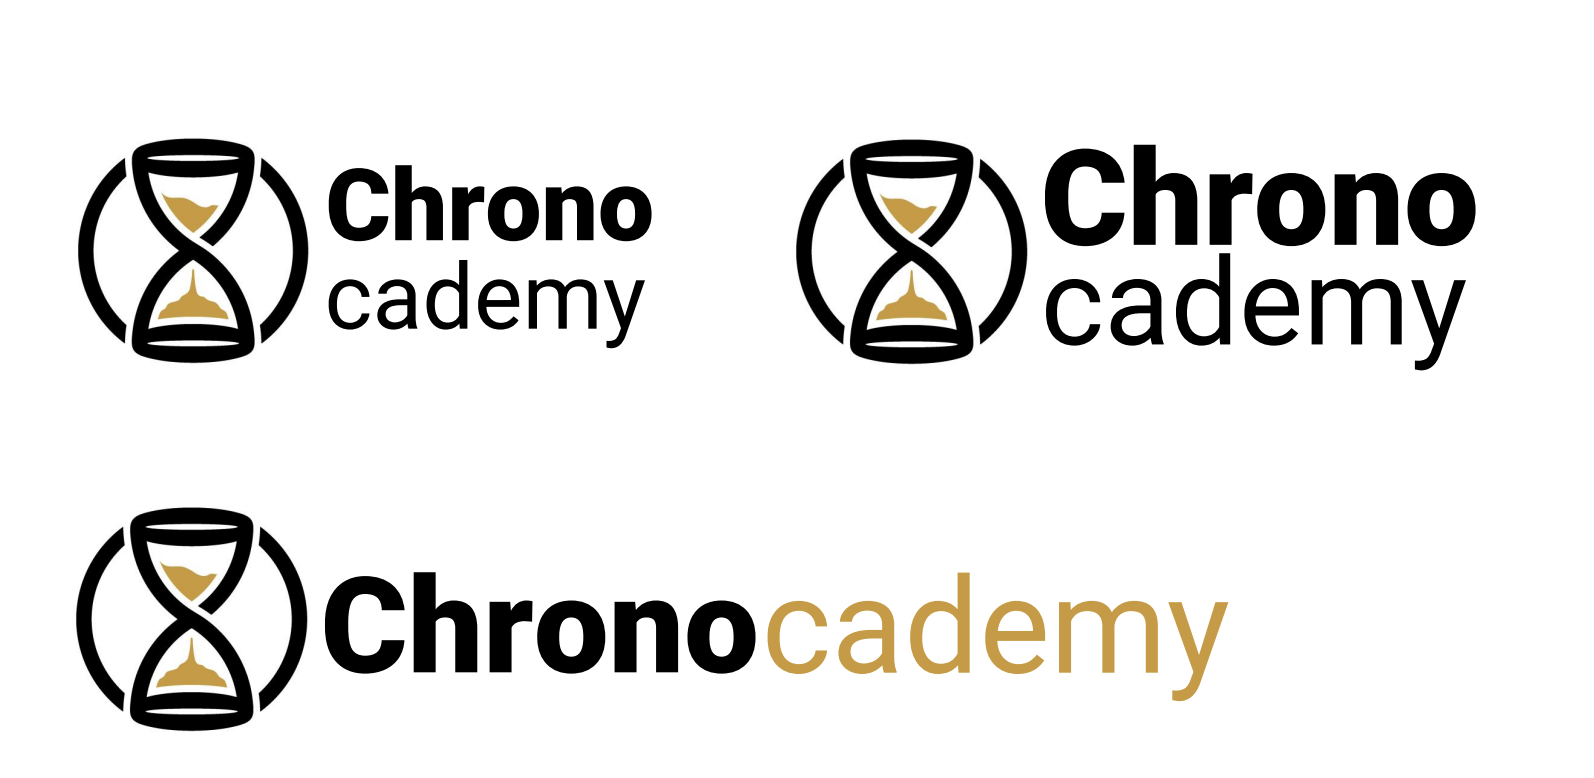
\includegraphics[width=10cm]{logo-iteration-1}
    \caption{Logo Option 1: The first option of the logo featured a stylized hourglass design with a bold, modern font.}
    \label{fig:figure4}
\end{figure}

\begin{figure}[h]
    \centering
    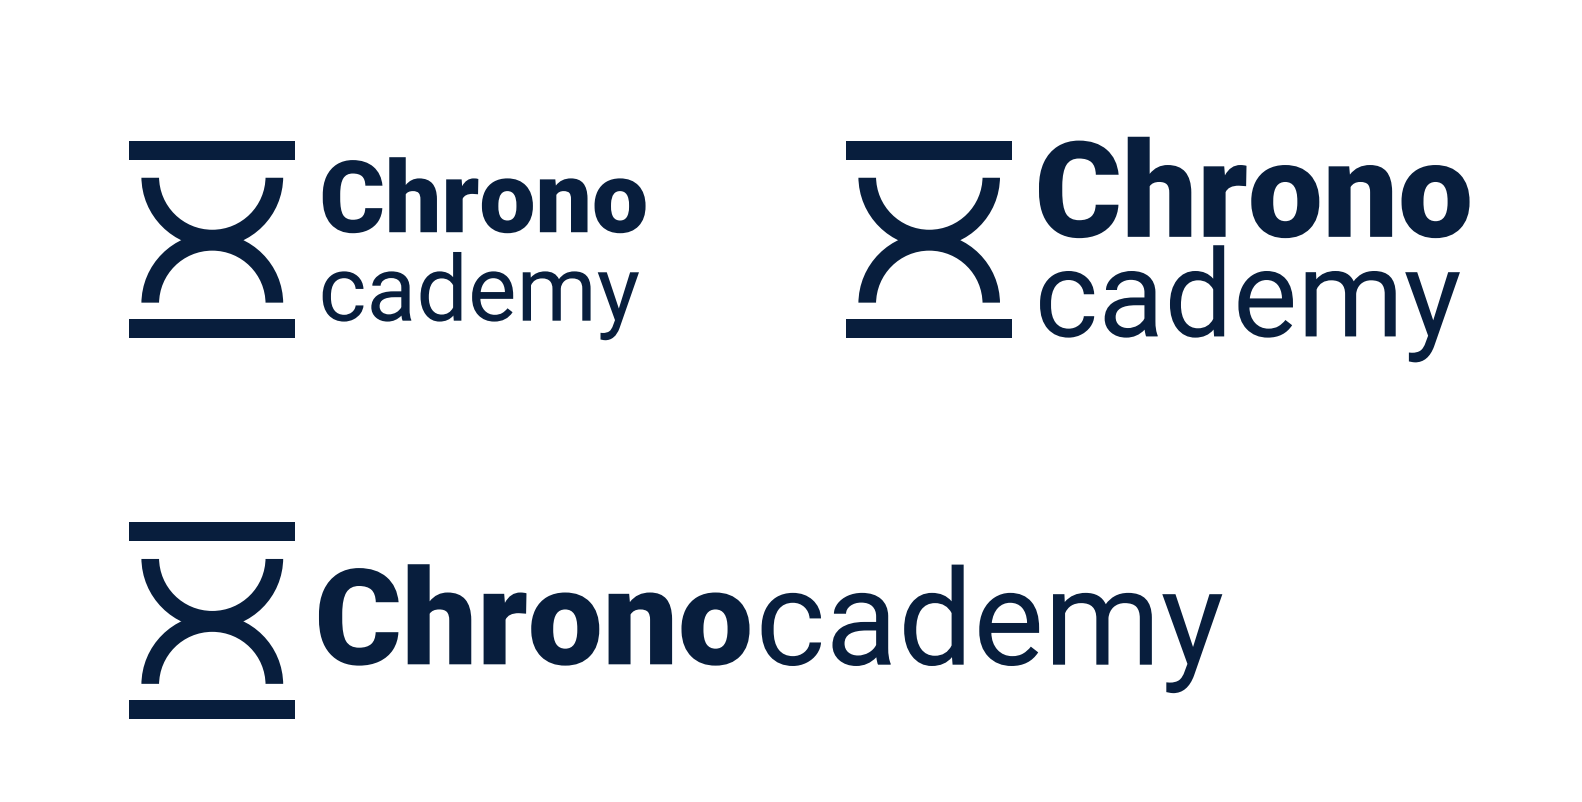
\includegraphics[width=10cm]{logo-iteration-2}
    \caption{Logo Option 2: The second option has a more modern and minimalistic hourglass and almost the same font properties.}
    \label{fig:figure5}
\end{figure}

\noindent There were actually many more iterations of the logo, but these two were the ones that were considered to be the most promising.
The reader can find all the iterations in the appendix.
\clearpage

\begin{figure}[t]
    \centering
    
\includegraphics[width=8cm]{logo-final}
    \caption{The final logo was a combination of the second option's hourglass and the first option's font.}
    \label{fig:figure6}
\end{figure}

\subsubsection{Slogans}\label{subsubsec:slogans}
The team brainstormed several slogans that encapsulated the essence of Chronocademy and its value proposition.
After careful consideration, the following slogans were selected:
\begin{itemize}
    \item \textbf{``Where you can: Learn. Teach. Grow.''}: This slogan captures the core activities of the platform, emphasizing the cyclical nature of learning and teaching.
    It conveys the idea that users can continuously expand their knowledge, share their expertise, and develop new skills through the platform.
    \item \textbf{``Time is Knowledge.''}: This slogan highlights the platform’s unique time-based currency system, positioning time as a valuable resource for acquiring knowledge.
    It underscores the platform’s focus on real-time learning experiences and the exchange of time for educational growth.
    \item \textbf{``Empowering Learning, One Hour at a Time.''}: This slogan emphasizes the platform’s commitment to empowering users through accessible, flexible learning opportunities.
    It communicates the idea that users can take control of their learning journey, one hour at a time, and achieve personal and professional growth through the platform.

\end{itemize}

After these three slogans were selected, we started to think how the slogan would match the logo and color palette to create a consistent brand.
The final decision was to break them into smaller parts and extract what we thought was useful for the brand.
For example, from the the second slogan, we extracted ``knowledge'' and instead of saying ``Time \textbf{is} Knowledge'' we thought that changing to ``Time \textbf{becomes} Knowledge'' would be explicit enough to tell our users that they could become more ``knowledgeable'' by using the platform.
And from the first slogan, we liked how it transmits the idea of things \textbf{``through''} the platform, so we extracted the ``Where'' word and used it in the final slogan: \textbf{``Where time becomes knowledge''}.
\begin{figure}[h]
    \centering
    
\includegraphics[width=5cm]{logo-slogan}
    \caption{Logo with Slogan}
    \label{fig:figure7}
\end{figure}

\subsection{Defining the Target Audience}\label{subsec:target-audience}

The third step in the product development process was identifying the target audience for Chronocademy, including their characteristics, preferences, and strategies for attracting and retaining them.
The target audience consists of the following groups:

\begin{itemize}
    \item \underline{Learners Only}: These users are interested in acquiring new skills but have no interest or time to teach.
    They prefer structured, face-to-face learning with specific goals in mind and have the financial means to purchase Chrono tokens.
    Strategies to attract them include highlighting the option to buy Chronos and showcasing the platform’s variety of classes and user-friendly features.
    Retention methods include offering high-quality courses, loyalty programs, progress tracking, and a community space for sharing experiences.
    \item \underline{Teachers Only}: These users focus on sharing knowledge and earning Chrono but are not interested in learning.
    They are often experienced educators motivated by the flexibility and financial incentives of the platform.
    To attract them, the emphasis should be on earning Chronos, success stories, and ease of use.
    Retention strategies include resources for teaching improvement, certifications, and a supportive community.
    \item \underline{Teachers and Learners}: This group enjoys both learning and teaching, motivated by personal development and the opportunity to share knowledge.
    Attracting them requires emphasizing the dual benefits of earning and spending Chronos.
    Retention strategies focus on providing balanced incentives, such as personalized recommendations and recognition for active participation in both roles.
    \item \underline{Casual Learners}: These users are hobbyists learning for personal enjoyment without a structured schedule.
    They value flexibility and variety.
    Social media advertising and testimonials can help attract this group, while retention depends on expanding skill offerings and supporting flexible learning.
    \item \underline{Professional Learners}: These users aim to advance their careers or professional skills.
    They are willing to invest time and money for high-quality learning.
    Highlighting career benefits and using professional networks like LinkedIn can attract them, while retention relies on offering specialized teachers and networking opportunities.
    \item \underline{Casual Teachers}: These individuals teach for enjoyment or extra income without a professional teaching background.
    They are motivated by their passion for sharing knowledge.
    Strategies to attract them include emphasizing the rewarding aspects of teaching and using social media to engage hobbyists.
    Retention strategies mirror those for professional teachers but include additional support for casual teaching improvements.
    \item \underline{Professional Teachers}: Users with formal training or significant teaching experience who teach as a primary or secondary profession.
    Attracting this group involves promoting the platform’s quality assurance and advertising through professional networks.
    Retention focuses on recognition, networking opportunities, and featured promotions.
    \item \underline{Learners Without Money and Without Teaching Skills}: Users in this group want to learn but lack financial resources and teaching skills.
    Highlighting the free Chrono tokens for new users and offering opportunities to contribute non-teaching services can attract them.
    Retention strategies include incentives for alternative contributions and providing low-cost learning options.
    \item \underline{Referrers}: These users promote Chronocademy in exchange for rewards.
    A generous referral program, shareable promotional materials, and recognition for top referrers are key to attracting and retaining this group.
    \item \underline{Ambassadors}: Passionate users or influential individuals who represent Chronocademy and promote it within their networks.
    Attracting ambassadors involves direct outreach, exclusive benefits, and recognition for their contributions.
    Retention focuses on providing ongoing support, creating a sense of community, and rewarding their efforts through special privileges or events.
\end{itemize}

\subsection{Understanding the Problem: User Interviews and Feature Mapping}\label{subsec:user-interviews-feature-mapping}
To ensure that Chronocademy addressed a real pain / need, the team conducted interviews with potential users.
This exploratory phase involved gathering insights from individuals who were interested in learning new skills or sharing their skills.
The interviews showed common pain points, such as the difficulty of finding reliable teachers, the high cost of learning platforms, and the challenges of managing multiple tools for teaching and learning.
Using the feedback from these interviews, the team mapped user needs into actionable features for the platform.
For instance, the need for affordability led to the time-based currency model, while the desire for better teaching experiences led to the integration of scheduling and video conferencing tools.
This process ensured that every feature of Chronocademy was directly tied to solving a specific user problem.

To deep dive into this, three interviews were conducted with people that the team thought fulfilled or represent the target audience.
For privacy reasons, the names of the interviewees will not be disclosed but their profiles and learnings will be described:

\begin{itemize}
    \item The interviewee, a theater director and Greek teacher, shared his experience teaching online.
    He mainly teaches Greek and has occasionally taught theater, although theater is harder to teach online.
    He explained that the main reasons for teaching online are flexibility and convenience, as it saves time for both him and his students.
    He prefers one-to-one lessons because they are more effective, even though group classes can be more profitable.
    When choosing an online platform, he looks for ease of use, affordable advertising, and the platform’s popularity.
    He mentioned that some platforms, like SuperProf, became too expensive for students, which reduced his contacts.
    Feedback and ratings are important for building trust, but he is cautious with students who frequently complain about teachers.
    He is open to referral programs if there are benefits like free classes or money.
    After learning about Chronocademy, he liked the idea of earning Chronos to either cash out or use for other classes.
    He thought Denmark could be a good market because people there have the time and resources to teach and learn.
    He also stressed the importance of platform visibility and suggested reaching out to teachers from other platforms like SuperProf.
    Finally, he expressed interest in trying the Beta version of Chronocademy, especially if it offered benefits like premium features or starting Chronos.
    \item The interviewee, a sales representative and online english student, shared his experience learning online.
    He prefers face-to-face learning because it is more engaging and allows for immediate feedback.
    He has learned online: programming, English, and sales techniques.
    His main motivation for learning online is the flexibility, comfort, and the ability to learn from anywhere while growing professionally.
    He rather live classes than recorded ones because it allows him to follow his customised learning plan instead of an already defined one.
    Three features he values in an online platform are: reviews, punctual teachers, and the learning content / teaching level.
    He mentioned that online learning is more affordable and flexible than traditional classes.
    The digital tools he uses while learning online are: Word, for notes; Conference platforms, for classes; and other websites with exercises the teacher might suggest.
    After learning about Chronocademy, he liked the idea of Chrono currency but he suggest it should be very clear from the beginning how it works and provide full transparency and trust to the users.
    \item The interviewee, an English language teacher shared her experience teaching online.
    She has an physical english academy in San Luis, Argentina and an online business unit as well.
    She is currently trying to expand the online side to Spain, since the physical side on Argentina cannot scale anymore.
    The current infrastructure of her online business is a landing page, Instagram account (social media) and online classes via Zoom (online conferencing platform).
    She and her employees only teaches English and Spanish languages but she said she could add ``coaching'' and ``online business consultant'' to the list of online services.
    Two big benefits she finds in her online business are the ability to record employee's onboarding and training sessions and class recordings for missing students.
    While one ``big'' trade-off is that she believes online learning is not for everyone since all her +50 years old students, struggle to interact with the digital tools.
    Based on her experience, group classes are more engaging and profitable than individual classes.
    ``Zoom'' technology is better than ``Google Meet'', she has tried both paid tiers.
    After hearing about Chronocademy's vision and intention with the time-based currency ``chrono'' she does not believe it will work since every language teacher she knows would charge for their work.
    Some advice from her is paying attention to user's technical issues while learning online, the digital skills of our target audience and improving online group learning technologies.
\end{itemize}

\newpage
\subsection{Competitor Analysis}\label{subsec:competitor-analysis}
The fifth step in the product development process was conducting a competitor analysis to understand the strengths and weaknesses of existing platforms.
This analysis involved identifying direct and indirect competitors, evaluating their features, pricing, user experience, and market positioning.
The team researched platforms such as SuperProf, Preply, and Tandem to gain insights into the online learning landscape.

\subsubsection{Direct competitors}

For these three main competitors, we picked some of their main features and analyzed each of this in detail, focusing on the things they got right and what we believe they got wrong.
The analysis was based on these main features for each platform:
\begin{itemize}
    \item User profile creation
    \item Premium plan
    \item Page navigation
    \item How to find people to talk to
\end{itemize}

\paragraph{Tandem} is an online language learning platform that connects learners with native speakers worldwide for language exchange.
Its target audience includes language learners seeking to practice speaking with native speakers, as well as native speakers interested in practicing a foreign language and meeting new people.
The platform focuses exclusively on language learning and ensures quality through user ratings and reviews, optional identity verification, and community guidelines designed to promote respectful and productive exchanges.
Tandem adopts a monetization strategy that includes a free basic membership to attract users, a subscription-based premium service called Tandem Pro that offers features like an ad-free experience and advanced search filters, and in-app purchases, such as Tandem Coins for unlocking additional features or sending virtual gifts.
Its strengths include a global reach with a diverse user base, an intuitive and user-friendly interface, and an active community that fosters a supportive environment for language practice.
However, Tandem has some weaknesses, such as its exclusive focus on language exchange without offering structured courses or formal teaching methods, potential inconsistencies in the quality of user-driven exchanges, and limited accessibility for those unable to afford subscription fees or in-app purchases.

For this competitor, we focused on some of their main features and analyzed each of this in detail, focusing on the things they got right and what we believe they got wrong.
For example, in the picture attached below, the reader can see how we analyzed the sign-up / login process of Tandem, making notes on what we liked and what we would improve.

\begin{figure}[h]
    \centering
    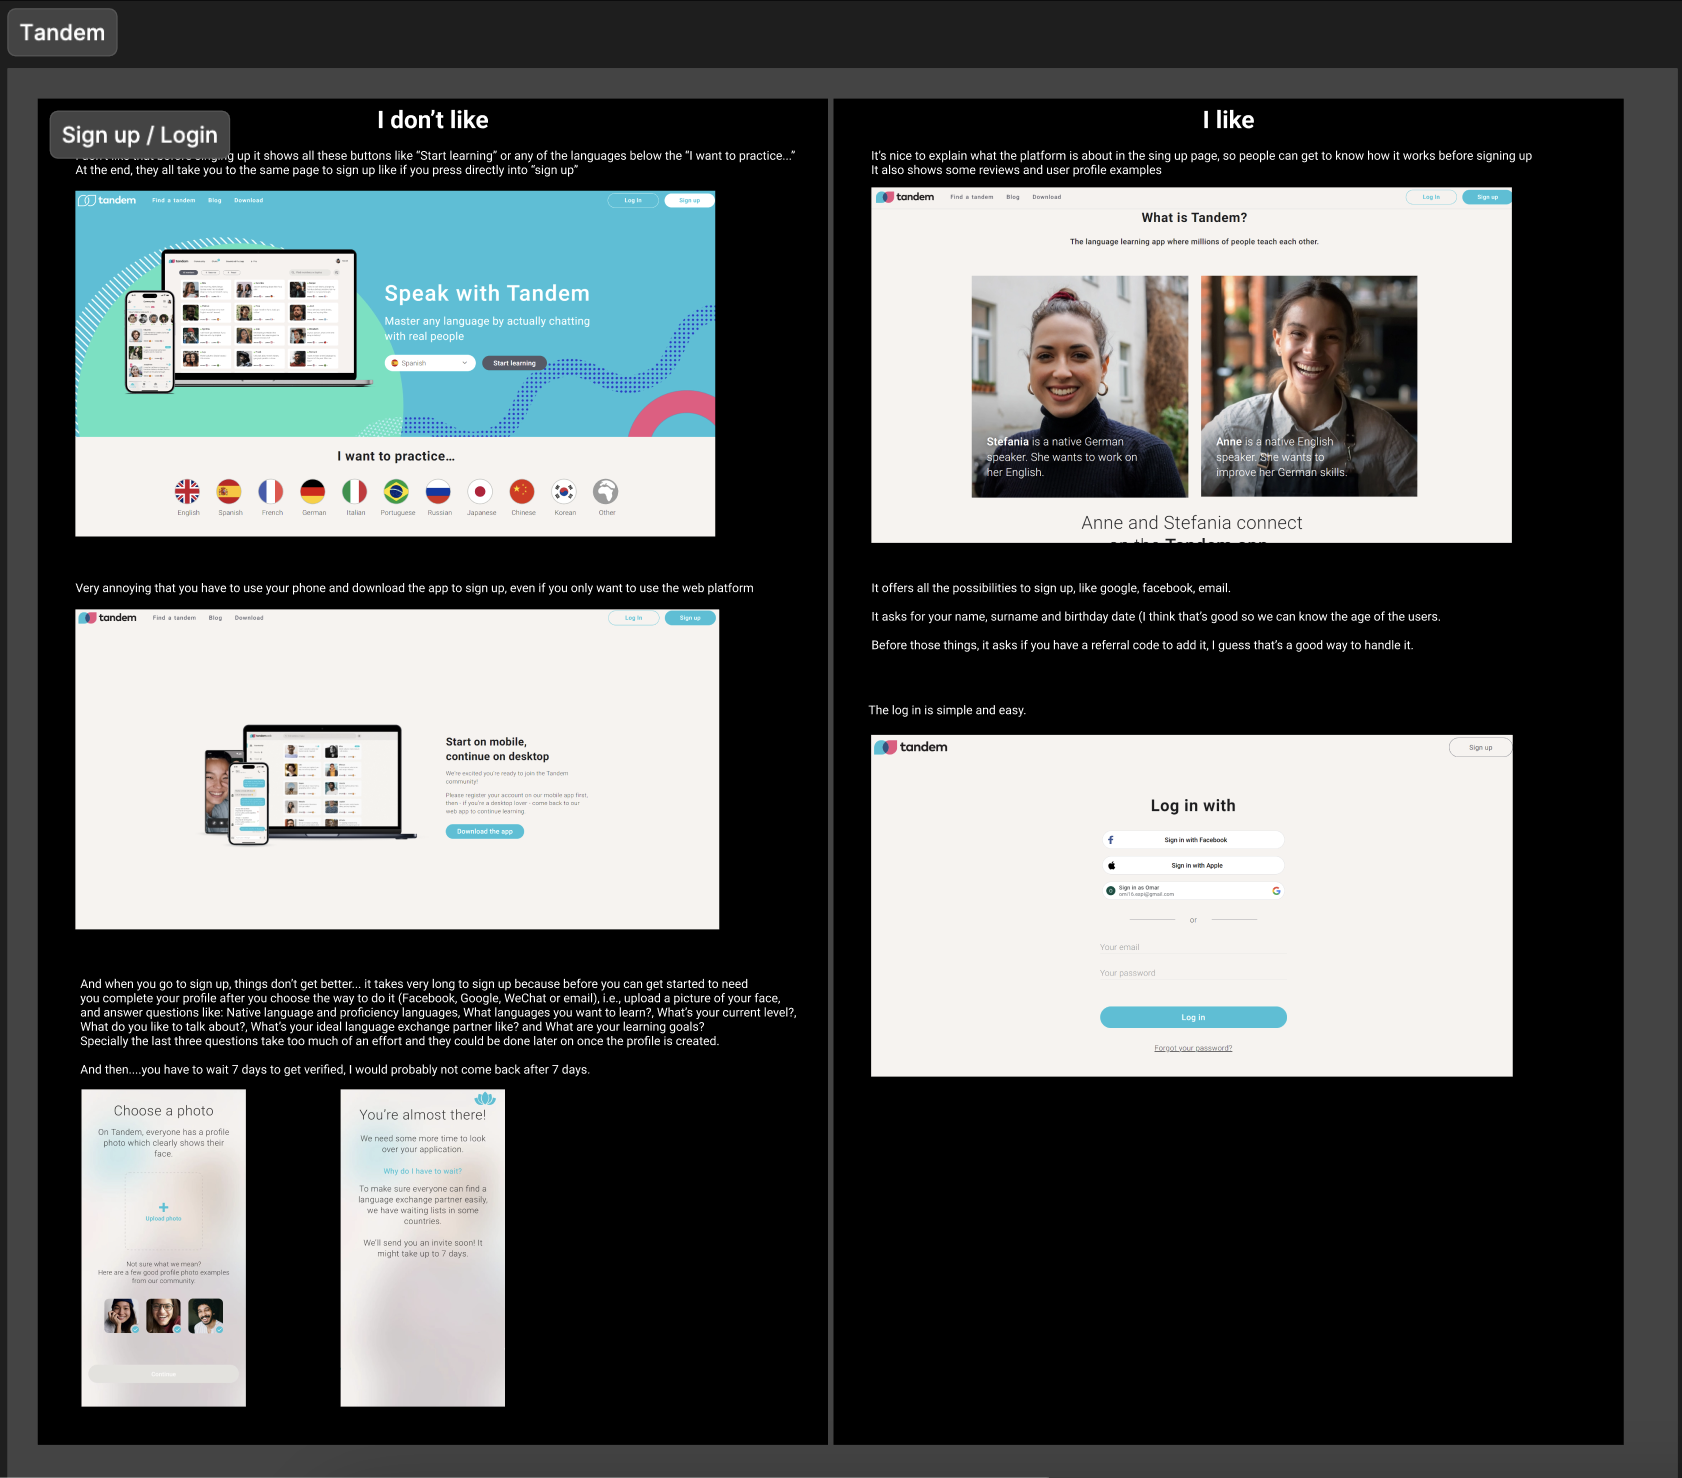
\includegraphics[width=14cm]{tandem-competitor-analysis}
    \caption{Tandem Competitor Analysis}
    \label{fig:figure8}
\end{figure}

\paragraph{SuperProf} is an online platform that connects students with tutors across a wide range of subjects and skills.
Its target audience includes learners seeking personalized instruction in academic subjects, hobbies, or professional skills, and tutors looking to offer their expertise to a global audience.
The platform supports a diverse array of course categories, encompassing everything from traditional school subjects to unique skills like yoga, music, and programming.
Quality control measures include user ratings and reviews to ensure reliable feedback, a tutor verification system to authenticate qualifications, and the option for tutors to provide introductory sessions to establish credibility.
SuperProf's monetization strategy revolves around subscription fees for tutors, who pay to list their services and gain visibility, while learners typically access the platform for free, paying only for the classes they book.
Its strengths lie in its vast subject variety, user-friendly interface, and strong global presence, enabling learners to find tutors for nearly any subject.
However, weaknesses include a reliance on tutor subscriptions, which may discourage new or casual tutors, a lack of platform-wide standardized teaching methods, and potential challenges in ensuring consistent quality across its large and varied tutor base.
For this competitor, we examined some of their main features in detail, noting what they did well and areas for improvement.
For instance, in the image below, we analyzed Superprof's profile creation / edition, highlighting aspects we liked and potential enhancements.

\begin{figure}[h]
    \centering
    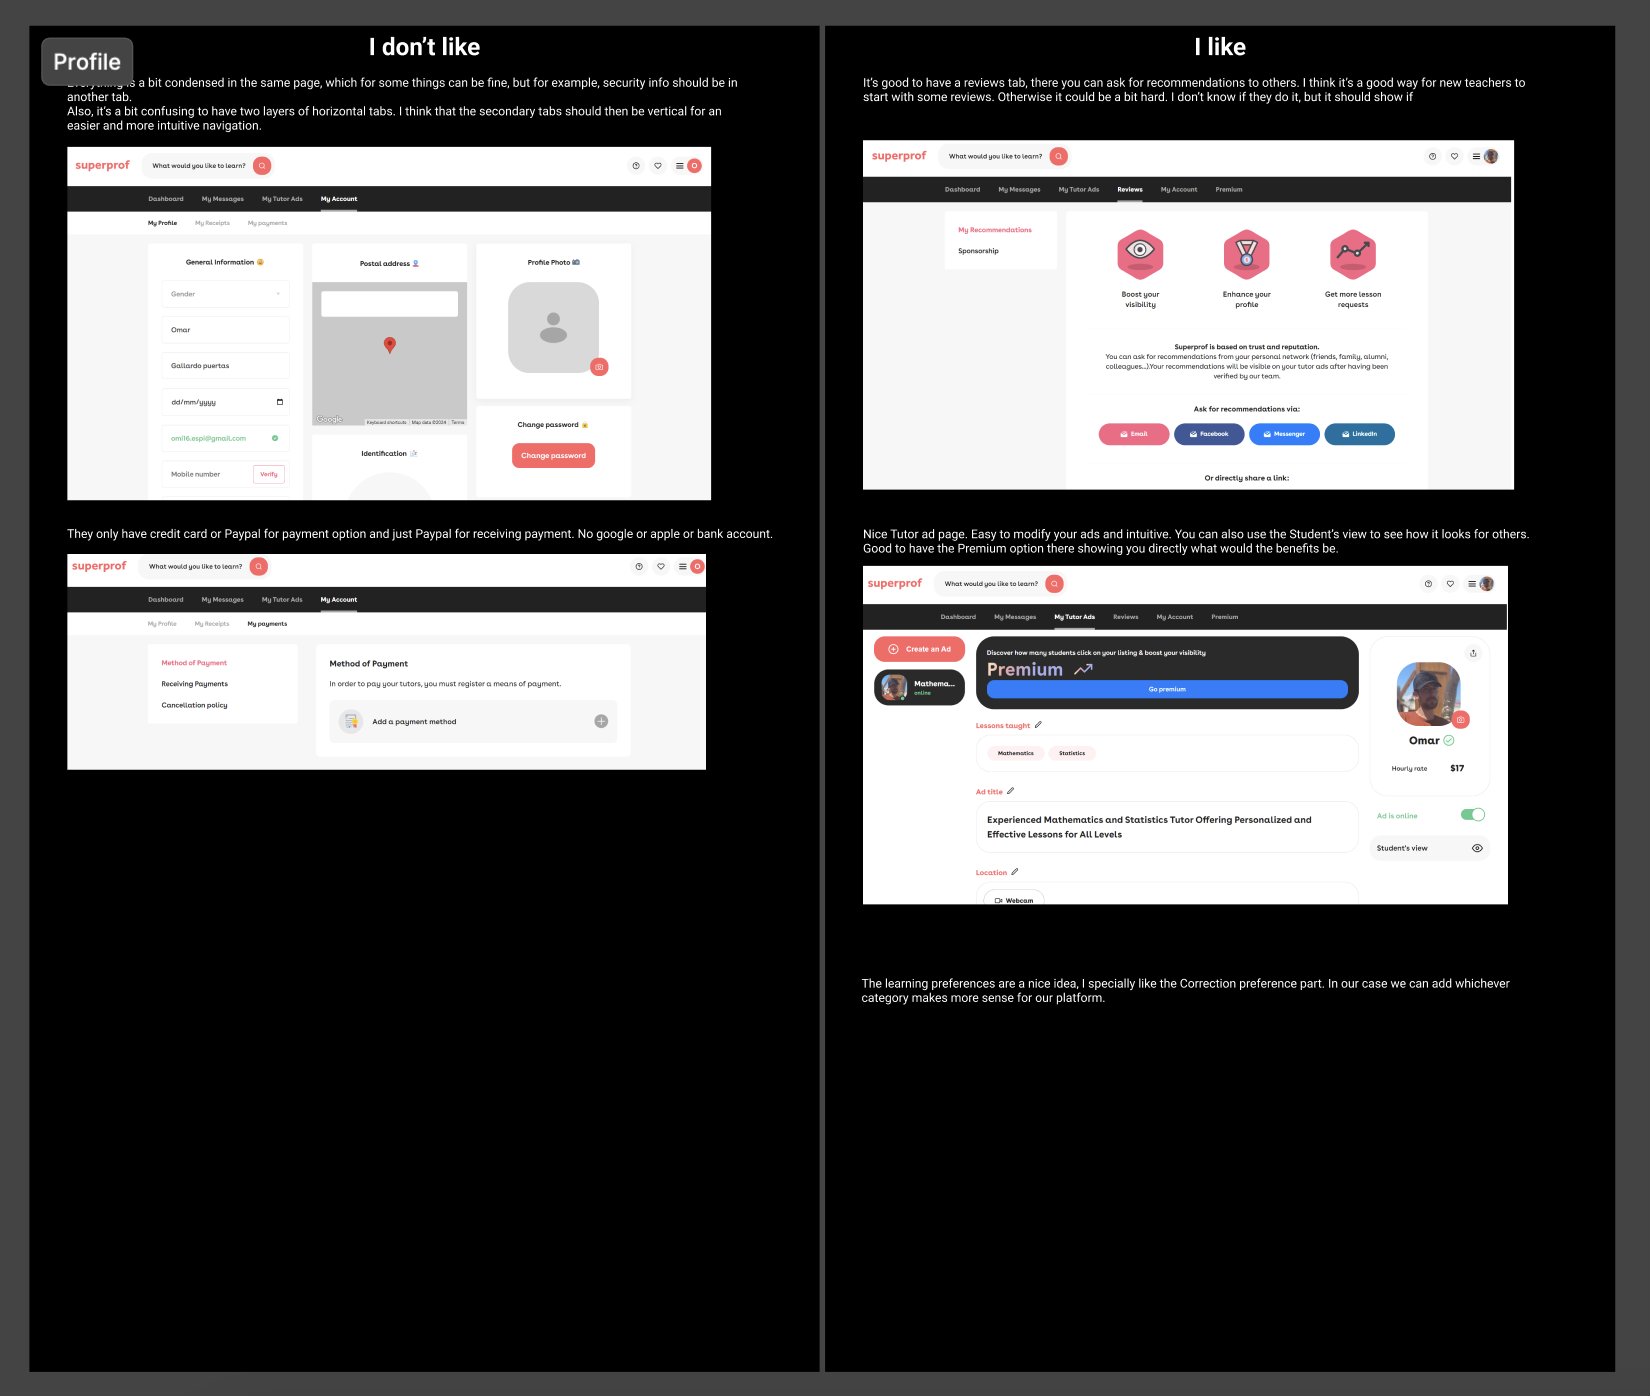
\includegraphics[width=14cm]{superprof-competitor-analysis}
    \caption{SuperProf Competitor Analysis}
    \label{fig:figure9}
\end{figure}

\paragraph{Preply} is an online platform that connects students with tutors for personalized one-on-one lessons in various subjects, with a strong emphasis on language learning.
Its target audience includes individuals seeking tailored instruction in languages, academic subjects, or professional skills, as well as tutors looking to monetize their expertise through flexible teaching opportunities.
The platform offers a diverse range of course categories, though it is particularly known for its language offerings.
Quality control measures include a tutor screening process, user reviews and ratings, and the ability for students to book trial lessons before committing to a tutor.
Preply's monetization strategy involves taking a commission from tutors' earnings, along with offering prepaid lesson packages that students purchase upfront.
Its strengths include a wide selection of qualified tutors, a user-friendly interface, and the flexibility of booking lessons tailored to individual schedules and goals.
However, weaknesses include the commission-based model, which may reduce tutors' earnings, and variability in the quality of tutoring experiences due to its user-driven nature.
Additionally, the prepaid lesson system might deter students who prefer more flexible payment options.
For this competitor, we examined some of their main features in detail, noting what they did well and areas for improvement.
For instance, in the image below, we analyzed Preply's way of allowing users to find teachers, highlighting aspects we liked and potential enhancements.

\begin{figure}[h]
    \centering
    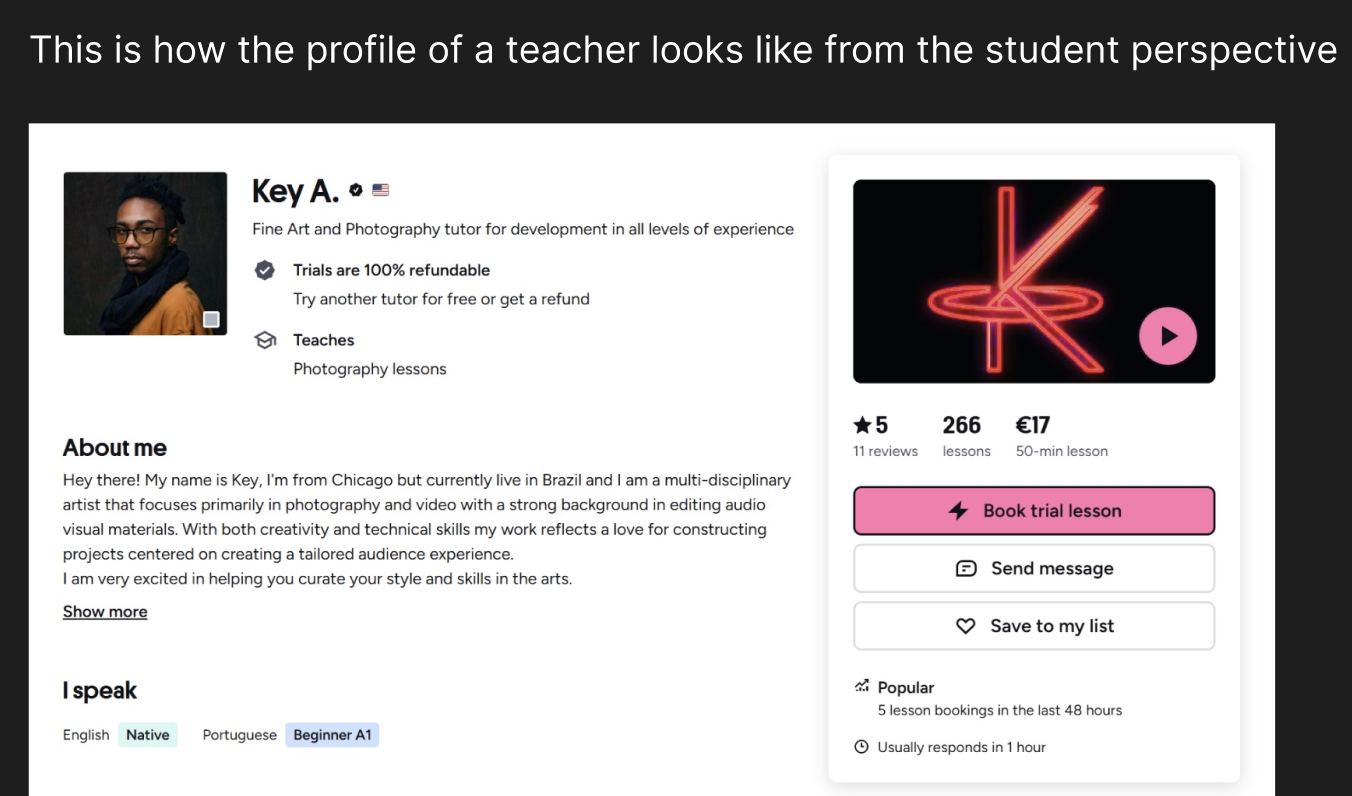
\includegraphics[width=14cm]{preply-competitor-analysis}
    \caption{Preply Competitor Analysis}
    \label{fig:figure10}
\end{figure}
\clearpage

\subsubsection{Indirect competitors}
Udemy, Coursera or Skillshare.
Online learning platforms that offer paid or subscription-based online courses.
Talkpal is an AI based platform where you can use an ai teacher for different levels.
They still need to improve, but they will be a direct competitor in the future.
Duolingo, online platforms to learn languages by practicing and repetition, but without human interaction.

\subsubsection{Competitive Advantages}
\begin{itemize}
    \item Time-based currency: This is a unique feature that can attract users looking for a more affordable and accessible learning experience compared to traditional paid courses.
    There is no need for initial investment for students if they don’t want to get a premium subscription.
    \item Focus on skill exchange: Chronocademy can create and grow a community-driven atmosphere where users can share a wider range of skills beyond what many online platforms might offer.
\end{itemize}
Flexibility: The platform can help learners and instructors with busy schedules by managing their calendars and booking for classes.
Also, since it’s online, there isn’t commuting time neither for the teacher or student.

\subsubsection{Challenges and Considerations}
\begin{itemize}
    \item Maintaining quality control: Ensuring instructors deliver valuable and accurate lessons requires well-defined or robust feedback mechanisms and moderation.
    \item Motivating instructors: Without immediate financial rewards, Chronocademy needs to create a system that incentivizes instructors to share their knowledge and maintain a high level of engagement.
    \item Critical mass: The platform needs to attract a sufficient number of users on both the learner and instructor sides to create a good learning ecosystem.
    \item Avoid fraudulent behaviours: The platform needs to be able to avoid fraudulent behaviours that can go either against the users or the company.
\end{itemize}

\subsection{Prioritizing Features with MoSCoW Priority Matrix and MVP with Lean Startup Approach}\label{subsec:prioritizing-features-with-the-lean-startup-approach}
After identifying potential features through user research and competitive analysis, the team needed to determine which ones were essential for the initial version of Chronocademy.
A feature list served as the blueprint for the platform, detailing everything Chronocademy needed to do—not only the core user-facing features but also the less visible technical requirements, such as single sign-on and potential API integrations like Google Meet.
This comprehensive approach ensured that both functional and technical needs were accounted for during development.
To prioritize these features, the team applied the Minimum Viable Product (MVP) methodology from the Lean Startup approach.
This method emphasized delivering a functional product with the core features necessary to provide value to users and validate the concept, while deferring non-essential elements to future iterations.

\begin{quote}
    ``A core component of Lean Startup methodology is the build-measure-learn feedback loop.
    The first step is figuring out the problem that needs to be solved and then developing a minimum viable product (MVP) to begin the process of learning as quickly as possible.
    Once the MVP is established, a startup can work on tuning the engine.
    This will involve measurement and learning and must include actionable metrics that can demonstrate cause and effect question.''
\end{quote}\cite[Lean StartUp]{leanStartUp}

By focusing on the essentials, the team was able to accelerate the development timeline and prepare for an earlier launch.
In parallel with this process, the team employed the MoSCoW prioritization matrix to further refine and validate feature decisions.
MoSCoW is a framework that categorizes project requirements into four levels of priority: Must have, Should have, Could have, and Would like but won’t get.
This method recognizes that while all features may seem important, only a subset is vital for immediate delivery and project success.\cite[Moscow Matrix]{moscowMatrix}
The ``Must have'' category represents the critical requirements without which the project would fail—these form the foundation of the MVP. For Chronocademy, the features that fell into this category and were prioritized for the initial release included:

\begin{itemize}
    \item Sign-up and login functionality,
    \item Course listings
    \item User profiles, enabling learners and teachers to interact, and
    \item Enable a communication channel between teachers and students.
\end{itemize}
Features categorized as ``Should have'' were considered valuable but not critical for the initial launch and were scheduled for future development.
``Could have'' features, such as advanced customization options and gamification elements, were acknowledged as desirable but non-essential and placed on a long-term roadmap.
Finally, features that landed in the ``Would like but won’t get'' category—those deemed too resource-intensive or offering minimal return on investment—were deprioritized and set aside for potential future consideration.

Competitive analysis also played a significant role in shaping the feature list.
By examining the branding, architecture, content, and feature sets of both direct and indirect competitors, the team identified which functionalities were essential for the initial release and which could differentiate Chronocademy from other platforms.
This process was not simply about replicating competitors’ features—rather, it revealed opportunities to address gaps in the market.
For instance, if competitors lacked flexible scheduling options, prioritizing that functionality immediately enhanced Chronocademy’s value proposition at launch.

This combined approach—leveraging both the MVP methodology and the MoSCoW matrix—not only allowed the team to focus on delivering core functionality quickly but also provided a structured framework for ongoing improvement.
Future feature development will be guided by user engagement metrics, feedback from early adopters, and the platform’s growth trajectory, ensuring that each new addition directly addresses user needs and enhances the Chronocademy experience.

\begin{figure}[h]
    \centering
    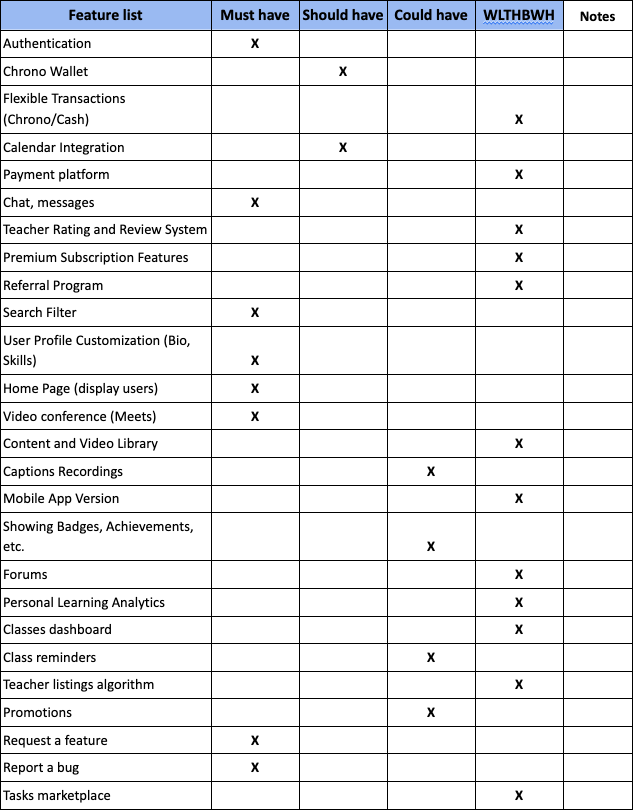
\includegraphics[width=14cm]{moscow}
    \caption{MoSCoW Priority Matrix}
    \label{fig:figure11}
\end{figure}

\subsubsection{MoSCoW Priority Matrix explained:}
After a thorough evaluation of the platform's requirements, we identified the essential features necessary to launch a Minimum Viable Product (MVP). These ``must-have'' features are critical for delivering core functionality and ensuring a seamless user experience.

\paragraph{Features included in the "Must Have" column:}
\begin{enumerate}
    \item Authentication – Essential for user access and security.
    \item Chat, Messages – Allows users to communicate directly on the platform.
    \item Search Filter – Enables users to find specific skills or people efficiently.
    \item User Profile Customization (Bio, Skills) – Allows users to showcase their skills and personal details.
    \item Home Page (Display Users) – Provides an overview of available users for skill exchange.
    \item Video Conference (Meets) – Facilitates virtual communication and lessons.
    \item Request a Feature – Allows users to suggest improvements.
    \item Report a Bug – Enables users to flag technical issues for better maintenance.
\end{enumerate}

\subparagraph{Decision on MVP Scope:}
Upon defining these critical features, we recognized that our initial vision for the MVP was too extensive.
To maintain focus and deliver a functional product efficiently, we decided not to include flexible payments or transactions (i.e., converting Chrono currency to cash) in this iteration.
Instead, our primary objective is to develop a simple skills exchange platform where users can connect, share their expertise, and engage in mutually beneficial exchanges.
This streamlined approach allows us to validate user interest and assess the platform's viability without the complexity of integrated financial transactions.
If we observe strong engagement and positive feedback from our user base, we will invest further resources to expand the platform.
Future iterations may incorporate additional features from the ``Should Have'', ``Could Have'', and ``WLTHBWH'' categories, including advanced payment solutions, calendar integration, and premium subscription features.
By focusing on the core exchange functionality, we aim to deliver a robust and user-friendly platform while remaining agile and responsive to market demands.
\clearpage

\section{User Experience Reasearch (UX)/ User Interface Design (UI)}\label{sec:user-experience-reasearch-(ux)/-user-interface-design-(ui)}
The user experience (UX) and user interface (UI) design of Chronocademy were critical components of the product development.
These aspects focused on creating an intuitive, engaging, and accessible experience for users, ensuring that the platform was easy to navigate, visually appealing, and functional.
This section outlines the research, design, and testing processes that guided the creation of Chronocademy's UX/UI\@.

\subsection{User Research}\label{subsec:user-research}
As mentioned above, user research was a foundational step in designing Chronocademy's UX\@.
This process involved understanding the needs, preferences, and behaviors of the platform's target audience to inform design decisions.
The team used the learning from the conducted interviews and the decided features as insights and feedback to shape the design.
To organize ourselves and our thoughts, the team followed some UX instruments that helped us to understand, document and prioritize our research:\newline
\begin{enumerate}
    \item Double Diamond: To guide the research and design phases.
    \item Value Proposition Canvas: To understand the user's pains and gains.
    \item User Personas: To create fictional characters that represent the target audience.
    \item User Flows: To understand the user's journey through the platform.
\end{enumerate}

For time constraints, the team could not conduct or utilize other research methods like:\newline
\begin{enumerate}
    \item User Journey Maps: To visualize the process a person goes through to accomplish a specific goal.
    \item Surveys: To gather quantitative data from a larger audience.
    \item Usability Tests: To test the platform with real users and gather feedback.
    \item High-Fidelity Prototypes: To test the platform with real users and gather feedback.
    \item A/B Testing: To test different versions of the platform and gather feedback.
    \item Design Systems: To create a consistent design across the platform.
\end{enumerate}

But the interviews were a good starting point to understand the user's needs and expectations, in combination with the competitor analysis, the team could gather enough information to start the design process.

\subsubsection{Double Diamond}\label{subsubsec:double-diamond}
To guide the design and development of Chronocademy, the team adopted the Double Diamond framework, a well-established model created by the Design Council.
This framework provides a structured approach to problem-solving and innovation by dividing the design process into four phases: Discover, Define, Develop, and Deliver.

\begin{figure}[h]
    \centering
    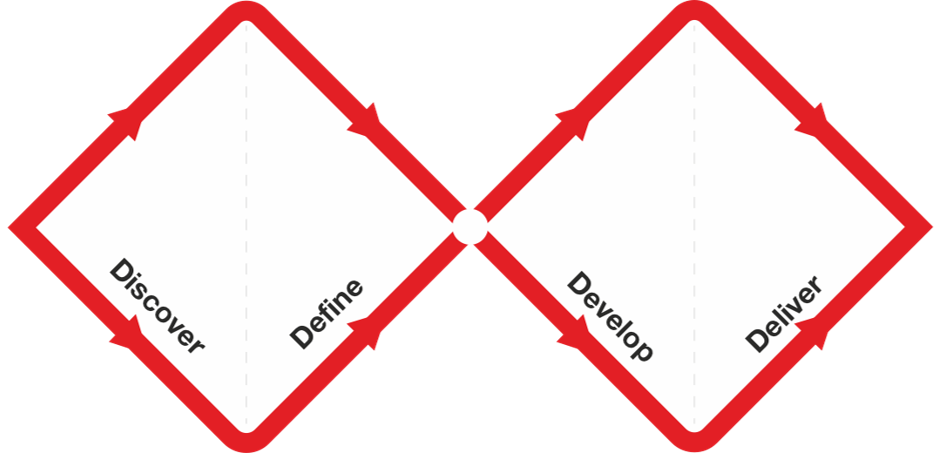
\includegraphics[width=14cm]{double-diamond}
    \caption{Double Diamond Framework}
    \label{fig:figure12}
\end{figure}
By definition, the Double Diamond is:
\begin{quote}
    ``A visual representation of the design and innovation process.
    It’s a simple way to describe the steps taken in any design and innovation project, irrespective of methods and tools used.''~\cite[Double Diamond]{doubleDiamond}
\end{quote}

\paragraph{Discover Phase:}
The implementation of this framework began with the Discover phase, which focused on user research and understanding the problems faced by both learners and educators.
During this one, we conducted the mentioned interviews and competitive analysis to gather insights into what users value in a learning platform.
For us, the main benefit of this tool, was that it brought order to the research process, helping us to organize our thoughts and prioritize our findings by adding a high level scope to the previously used and mentioned research methods.\newline

\paragraph{Define Phase:}
In the Define phase, we summarized the research findings into clear problem statements.
This phase involved organizing the data collected and identifying patterns to frame the core challenges Chronocademy aimed to solve.
A critical tool during this stage was the MoSCoW prioritization matrix, which we have previously discussed.
Another helpful tool was the Value Proposition Canvas, which helped us to align user needs with the platform's value proposition.
We will discuss this in more detail in the next section.
By converging on essential user needs, this phase ensured the team focused on solving the right problems without overcomplicating the MVP\@.\newline

\paragraph{Develop Phase:}
The Develop phase involved journey mapping and low level prototyping.
This stage embraced agile development practices, allowing the team to iterate rapidly while gathering user feedback.
On the product design side, the team created user flows, to map out the journey of our users through the platform.
We will discuss this in more detail in the next section.\newline
Another critical tool during this phase, was low fidelity prototyping, or wireframes.
These are simple, black and white sketches that help to visualize the layout of the platform and the placement of its elements.
Also, we will discuss this in more detail in the User Interface (UI) section.\newline

\paragraph{Deliver Phase:}
In the Delivery phase, the team finalized the core features and launched Chronocademy's MVP. This stage involved polishing the platform’s UI/UX, ensuring a seamless onboarding experience, and optimizing performance for real-world use.
The Double Diamond framework provided a clear way to balance exploration with execution.
It helped the team to:
\begin{itemize}
    \item Validate ideas through user-centered research.
    \item Prioritize effectively using the MoSCoW method.
    \item Iterate rapidly, ensuring a smooth and functional user experience.
    \item Deliver a robust MVP, focused on essential features while leaving room for future growth.
\end{itemize}
As we continue to refine Chronocademy, the Double Diamond framework remains an integral part of our continuous improvement process, ensuring the platform evolves based on real user feedback and emerging needs.
\clearpage

\subsubsection{Value Proposition Canvas}\label{subsubsec:value-proposition-canvas}
The Value Proposition Canvas is a tool that help businesses understand their customers' needs and desires, as well as how their products or services can meet those needs.
By definition, this diagram is:
\begin{quote}
    ``a tool for marketing experts, product
    owners, and value creators.
    This method from the bestselling innovation
    book Value Proposition Design is applied in leading organizations and
    start-ups worldwide.''~\cite[Value Proposition Canvas]{valuePropositionCanvas}
\end{quote}

It also helps to identify the user's pains and how the product can solve them, transforming them into gains and to achieve ``product-market fit''.\newline
\begin{quote}
    ``Product-market fit describes a scenario in which a company’s target
    customers are buying, using, and telling others about the company’s
    product in numbers large enough to sustain that product’s growth and
    profitability.''~\cite[Product Market Fit]{productMarketFit}
\end{quote}

The Value Proposition Canvas is divided into two main sections: the customer profile and the value map.
This is how the team filled the canvas for Chronocademy:

\begin{figure}[h]
    \centering
    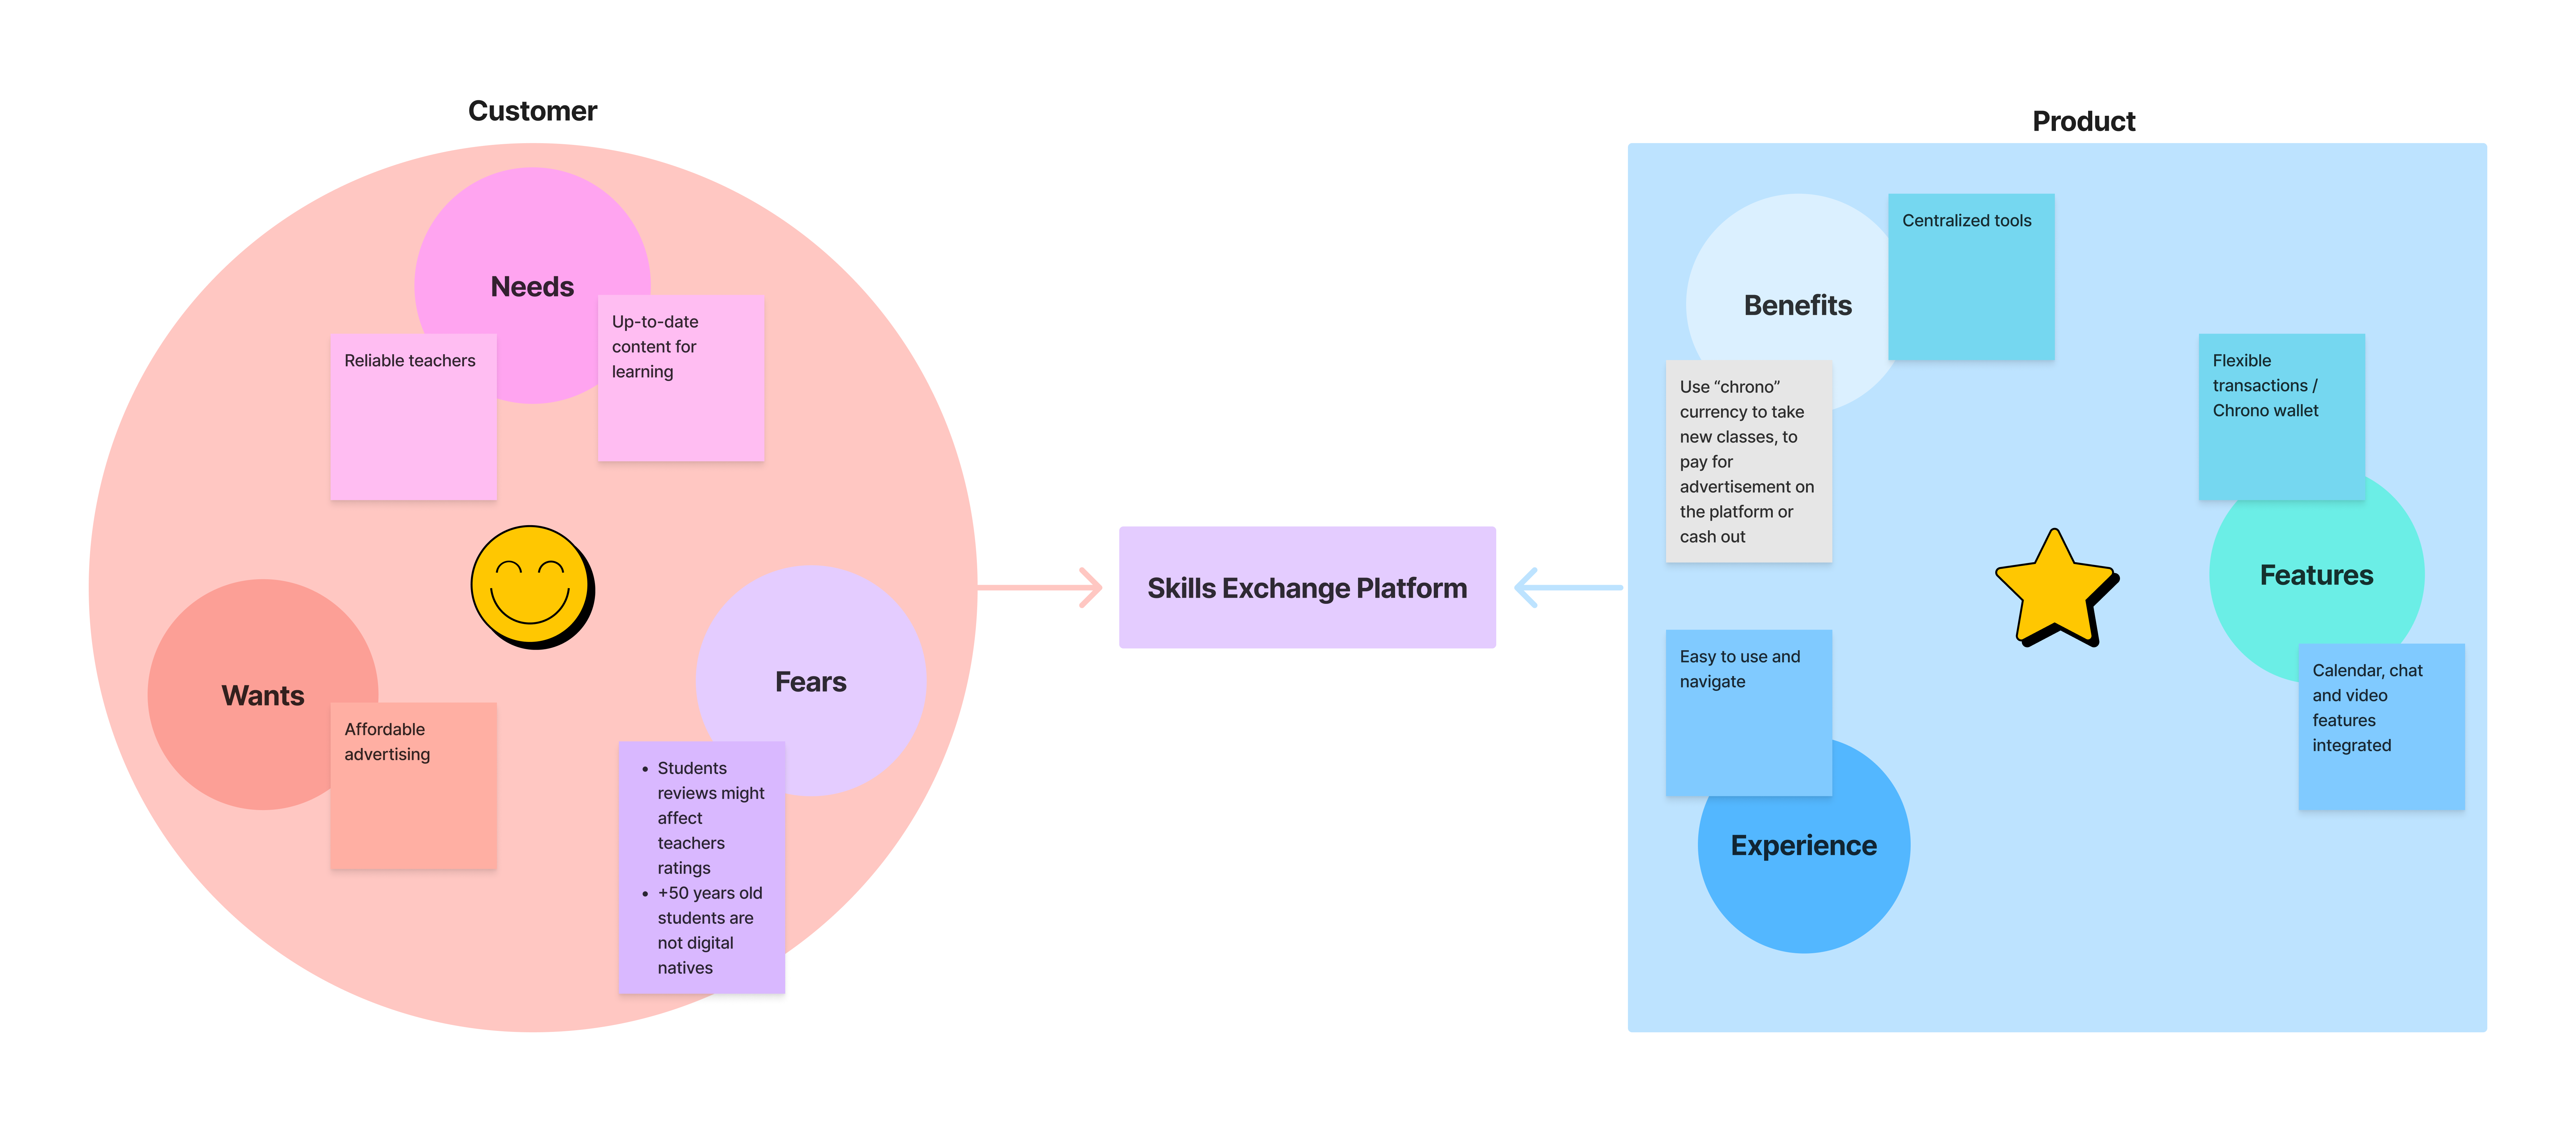
\includegraphics[width=13cm]{value-proposition-canvas}
    \caption{Value Proposition Canvas for Chronocademy}
    \label{fig:figure13}
\end{figure}

This canvas was built based on the insights gathered from the user interviews.
The main pains were extracted from the interviewees' feedback and the team's understanding of the platform's value proposition.
\begin{itemize}
    \item Reliable teachers (for students)
    \item Up-to-date content (for students)
    \item Affordable advertising (for teachers)
    \item Solid and reliable review's system (for both)
    \item Easy to use platform (for +50 years old students)
\end{itemize}
And were mapped to these gains in the form of features:
\begin{itemize}
    \item Flexible transactions (chrono)
    \item Easy to use platform - User centric design
    \item Reliable review system
    \item Centralized platform (video, calendar, chat integrations)
\end{itemize}

Overall, this canvas was a good starting point to understand the user's needs and expectations and to guide the design process during the ``Defne'' phase of the Double Diamond framework.
\clearpage

\subsubsection{User Personas}\label{subsubsec:user-personas}
User personas are fictional characters created to represent the different user types that might use a product or service.
They help to understand the needs, goals, and behaviors of potential users, guiding design decisions and ensuring that the product meets user expectations.
Quoting Qubstudio - Design Agency:
\begin{quote}
    ``A persona in UX is not the same as one in the market segment.
    It is a
    fictional character that represents overlapping patterns a large group
    of users demonstrates.
    It complements a digital product’s basement and
    is not affected by design changes or trends.''~\cite[User Personas]{userPersonas}
\end{quote}
So as mentioned before, these are not real users, but a representation of them.
It's typically based on user research, in our case, the conducted interviews.
After this, we tried to identify patterns and common issues that users might encounter.
And usually, designers try to make several user personas to represent a broader audience.\newline\newline
Some characteristics of a user persona are:
\begin{itemize}
    \item Name
    \item Age
    \item Job
    \item Goals
    \item Needs
    \item Pain points
    \item Behaviors
\end{itemize}

For Chronocademy, the team created four user personas to represent the different types of users that might interact with the platform.
We did not create more user personas, that would actually represent every type of user that could use the platform, because we wanted to focus on the MVP and the most common user types.
But the team could create more personas in the future, as the platform grows and more user types are identified.
Using this tool was very helpful because it allowed us to set the base for the design process and step by step begin the ``develop'' phase of the Double Diamond framework.

\begin{figure}[h]
    \centering
    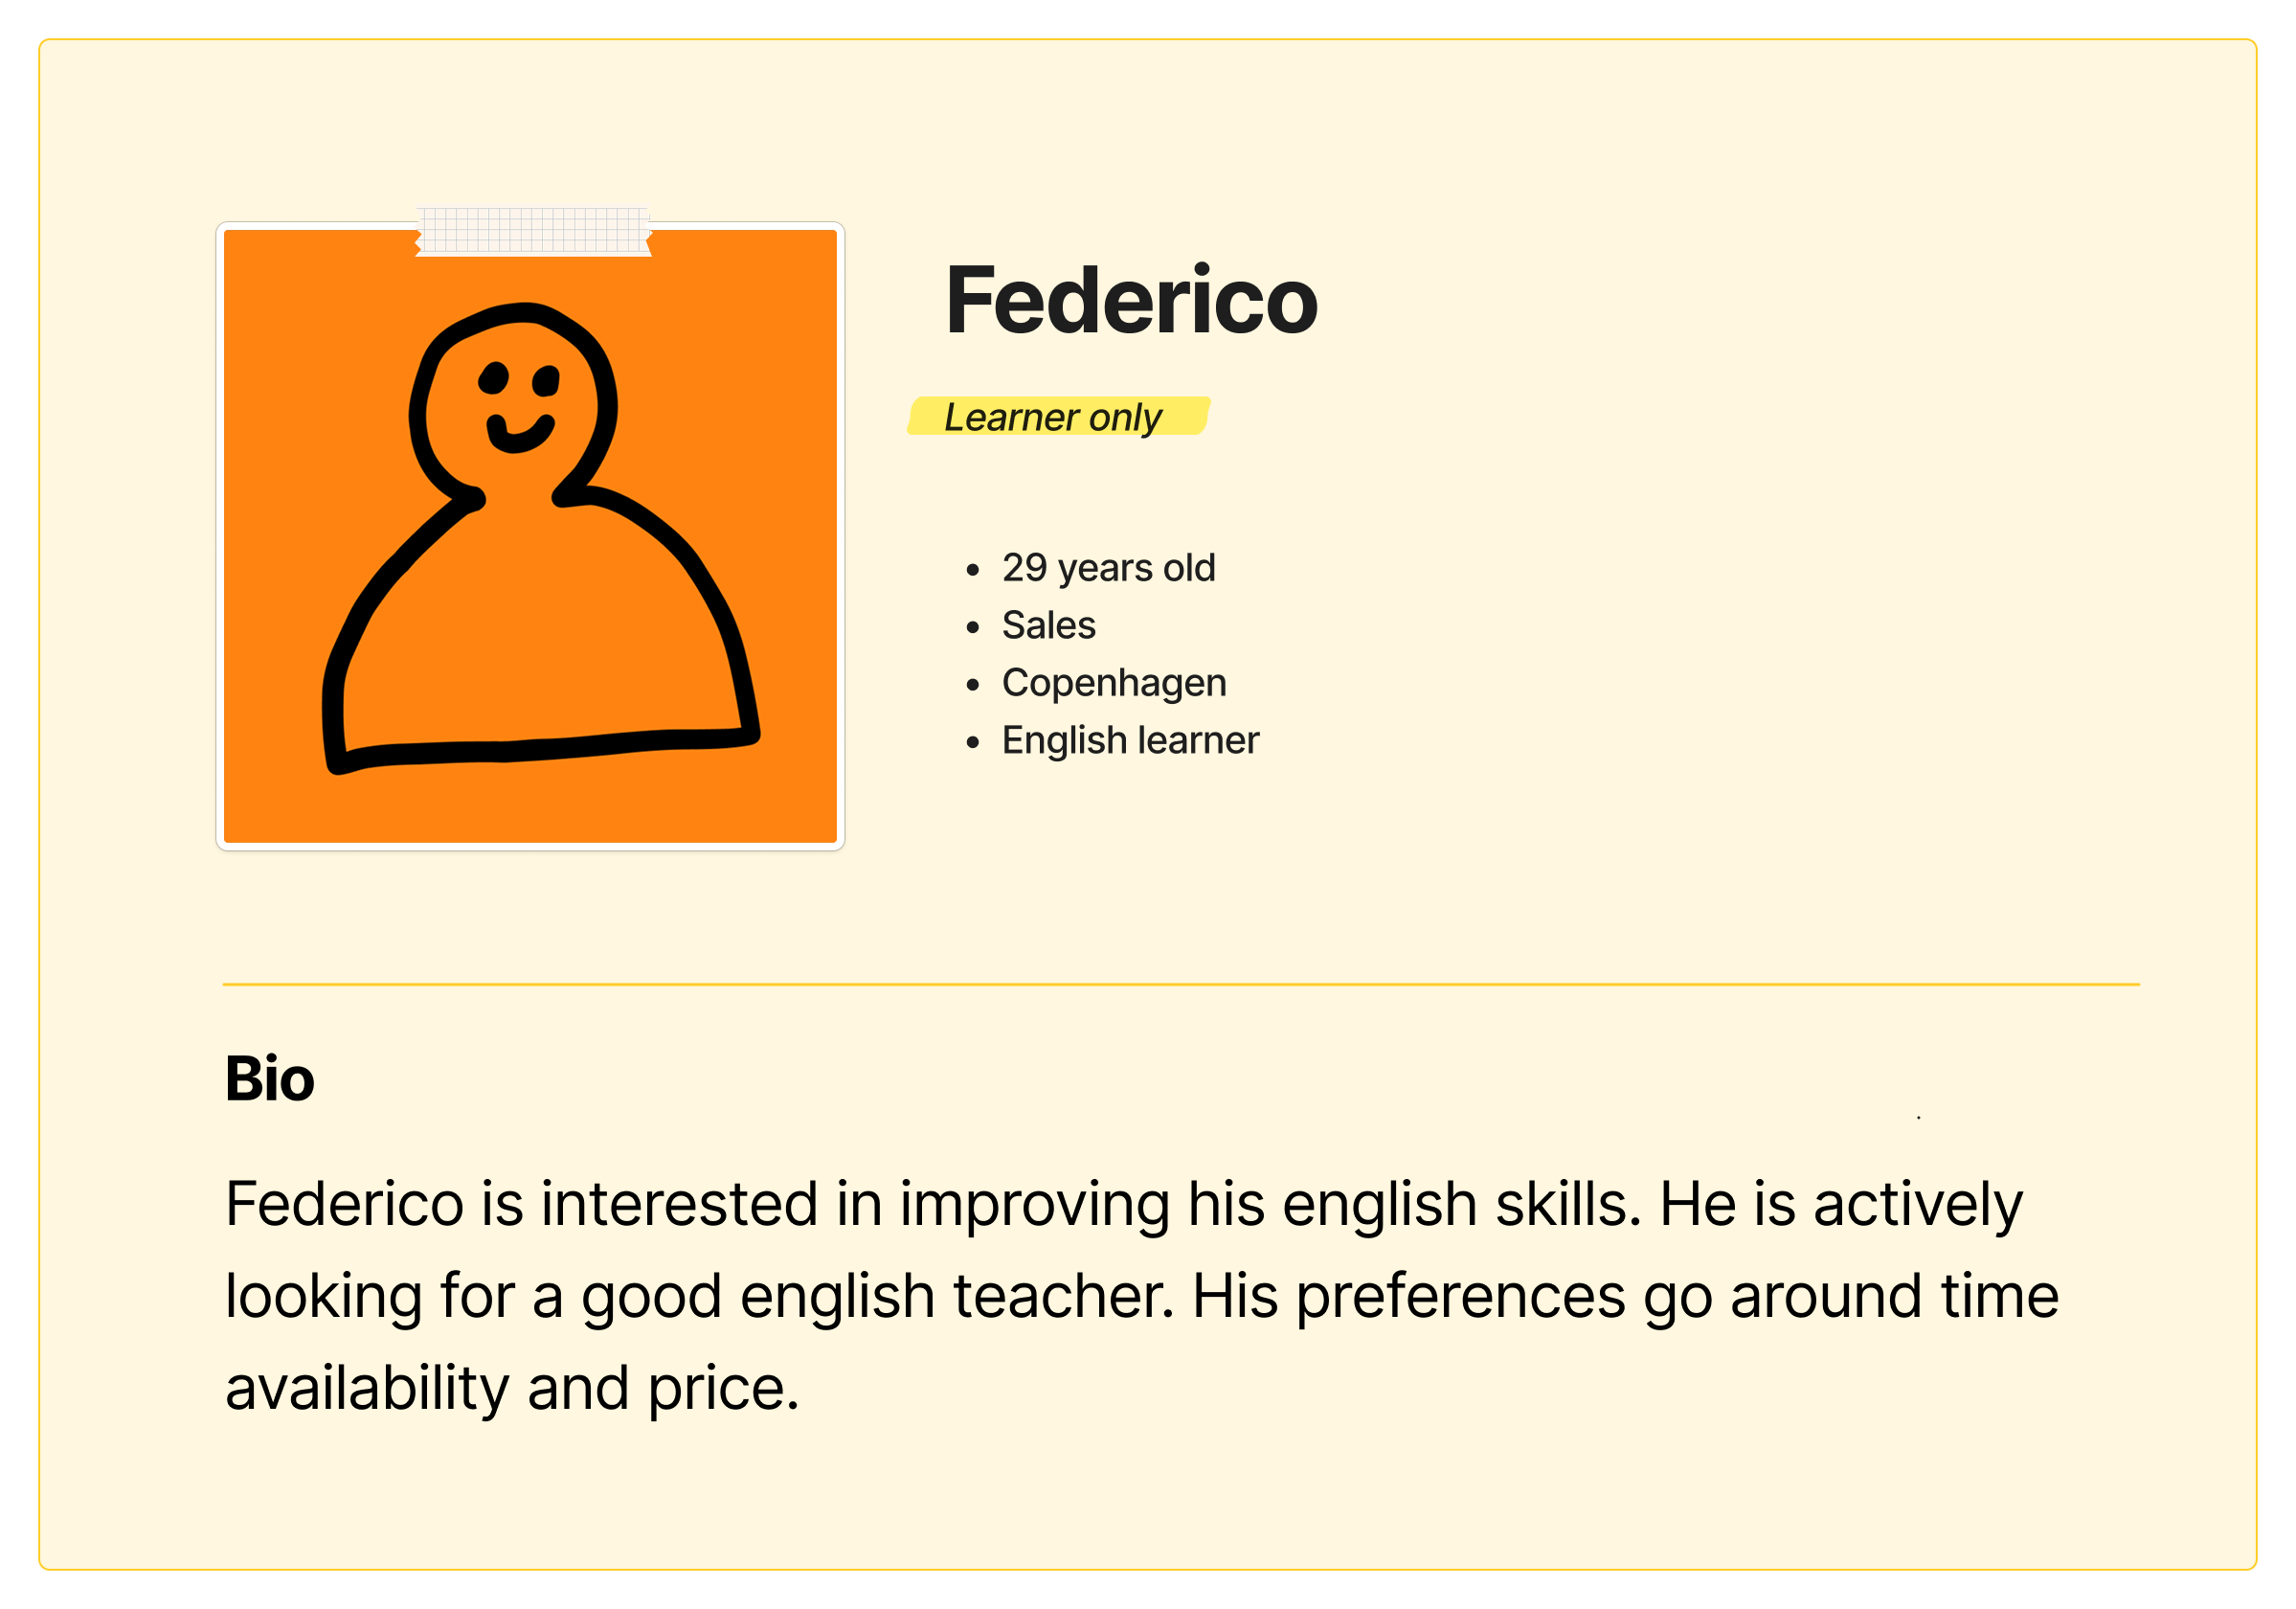
\includegraphics[width=10cm]{learner-only}
    \caption{A 29-year-old sales professional looking to learn new skills in their free time.}
    \label{fig:figure14}
\end{figure}
\begin{figure}[t]
    \centering
    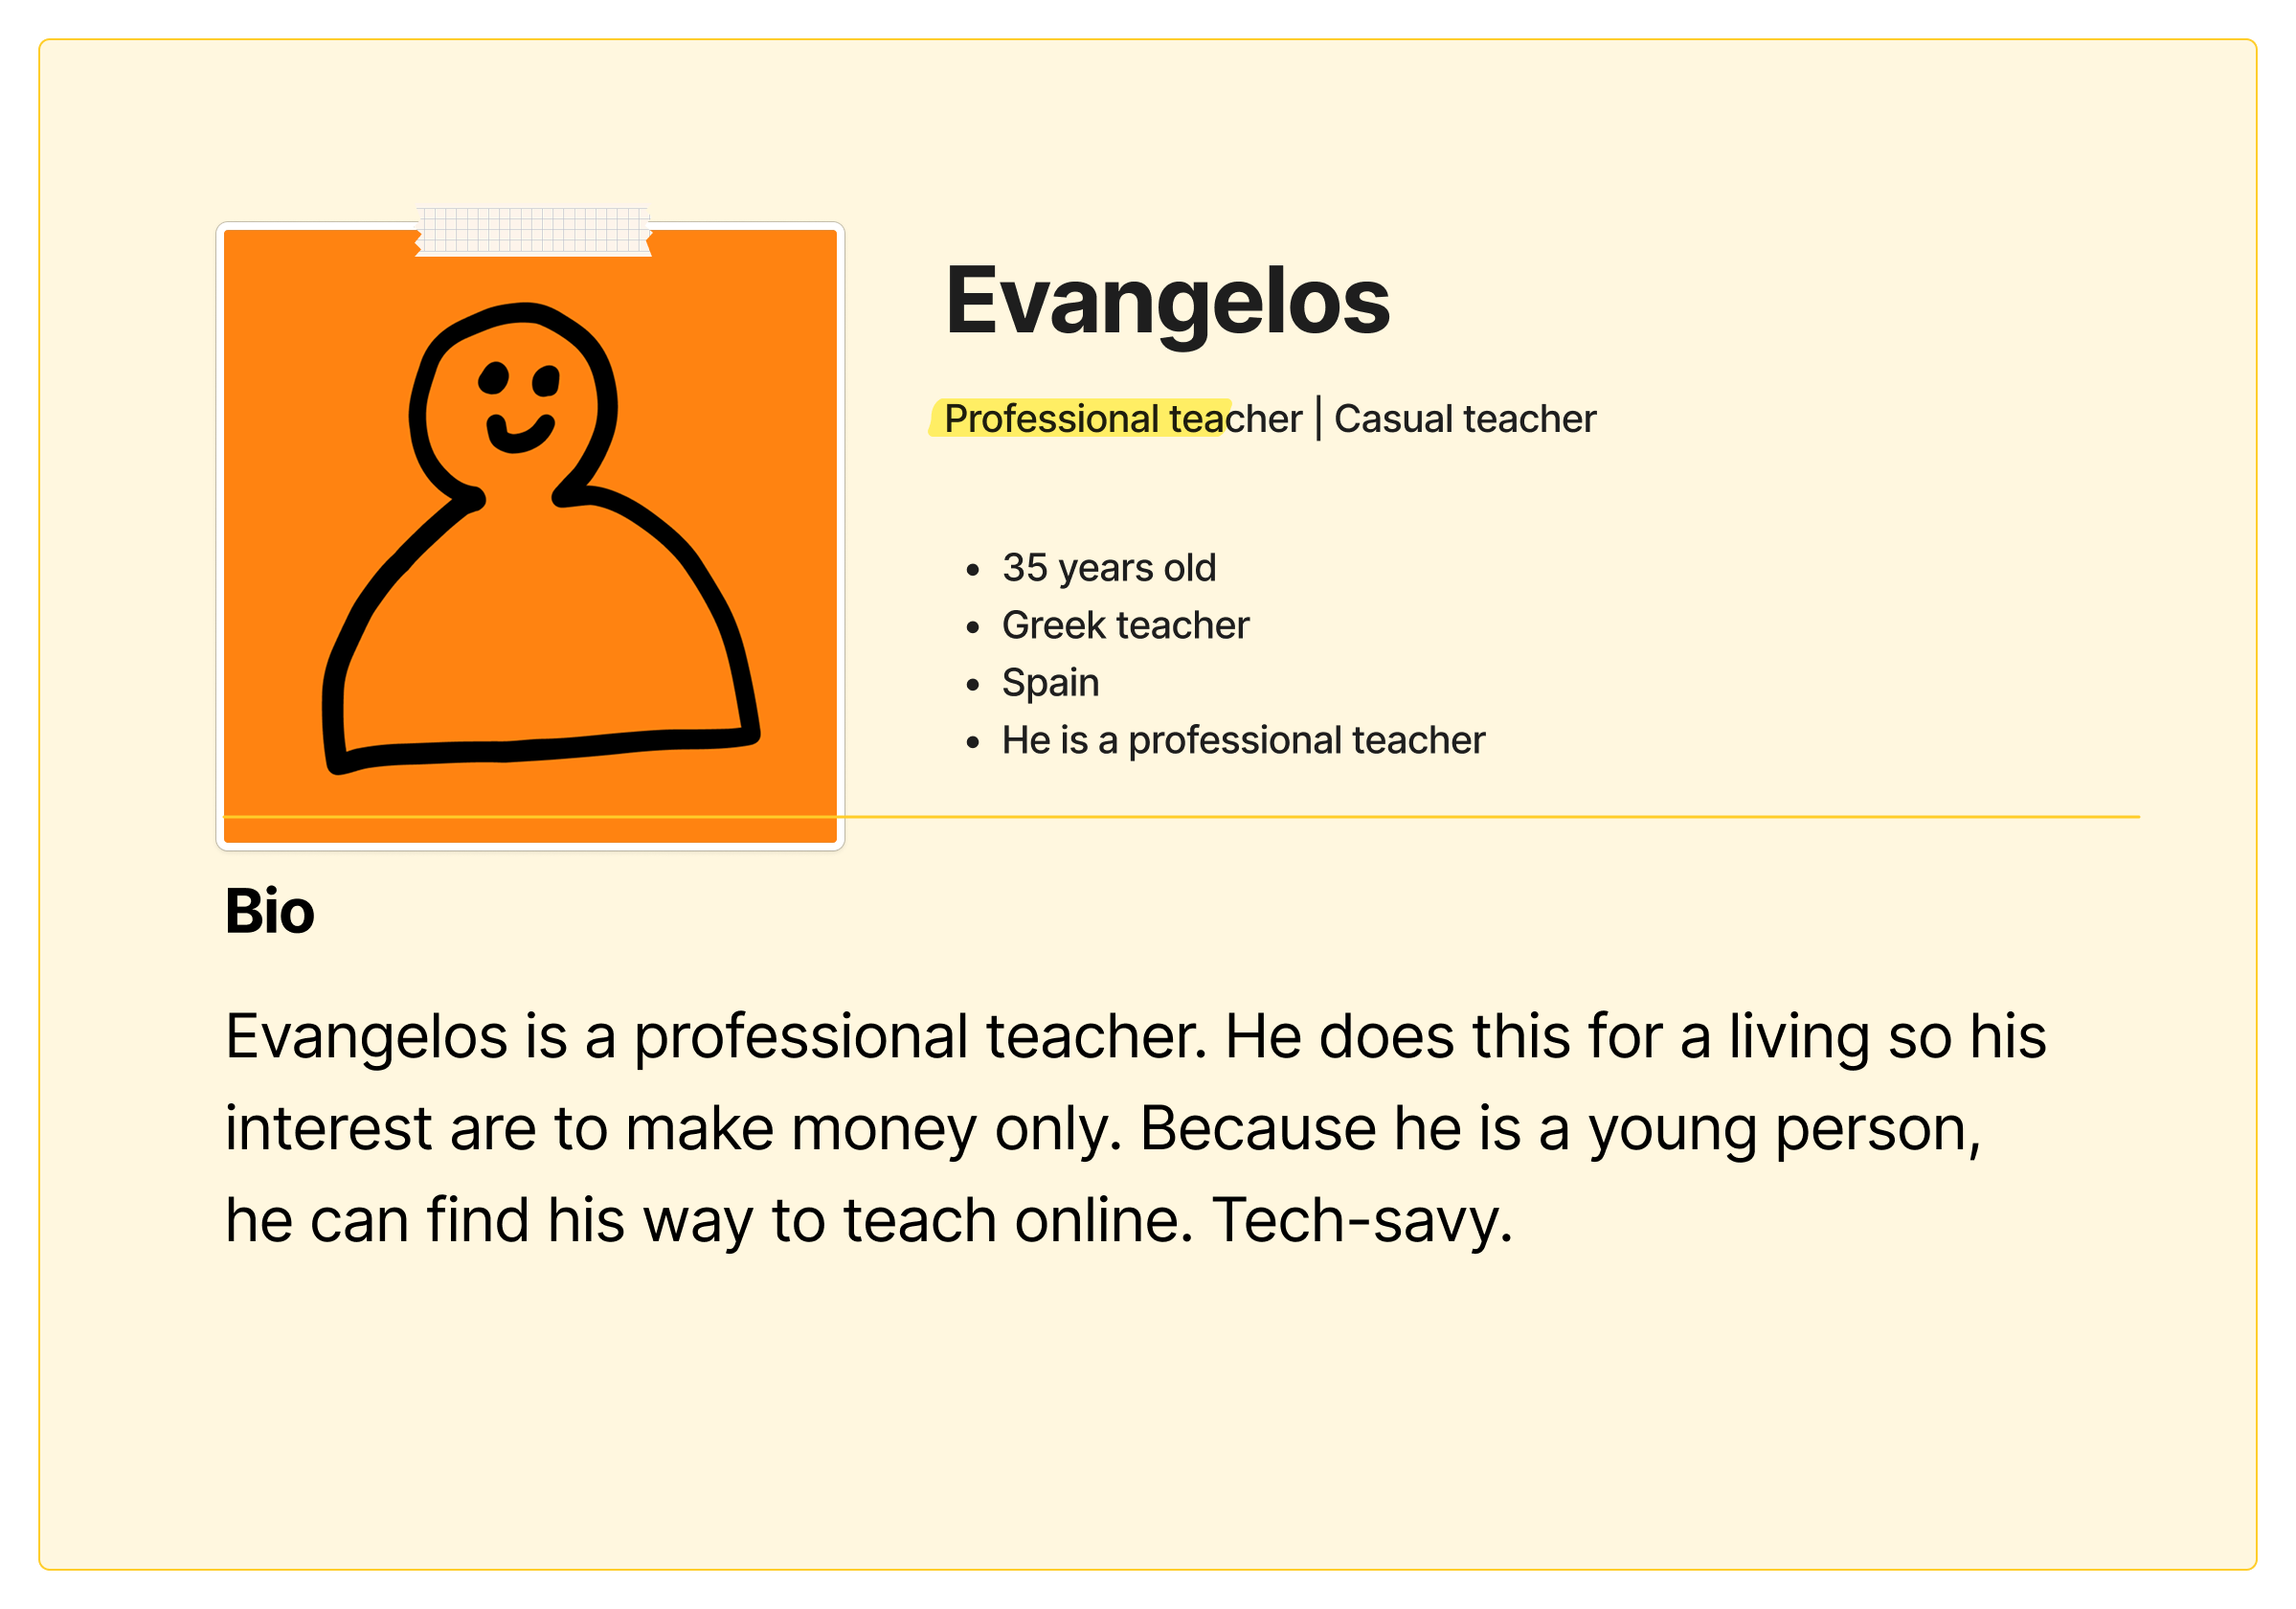
\includegraphics[width=10cm]{teacher-only}
    \caption{A 35-year-old language tutor seeking to expand his online teaching business.}
    \label{fig:figure15}
\end{figure}
\begin{figure}[h]
    \centering
    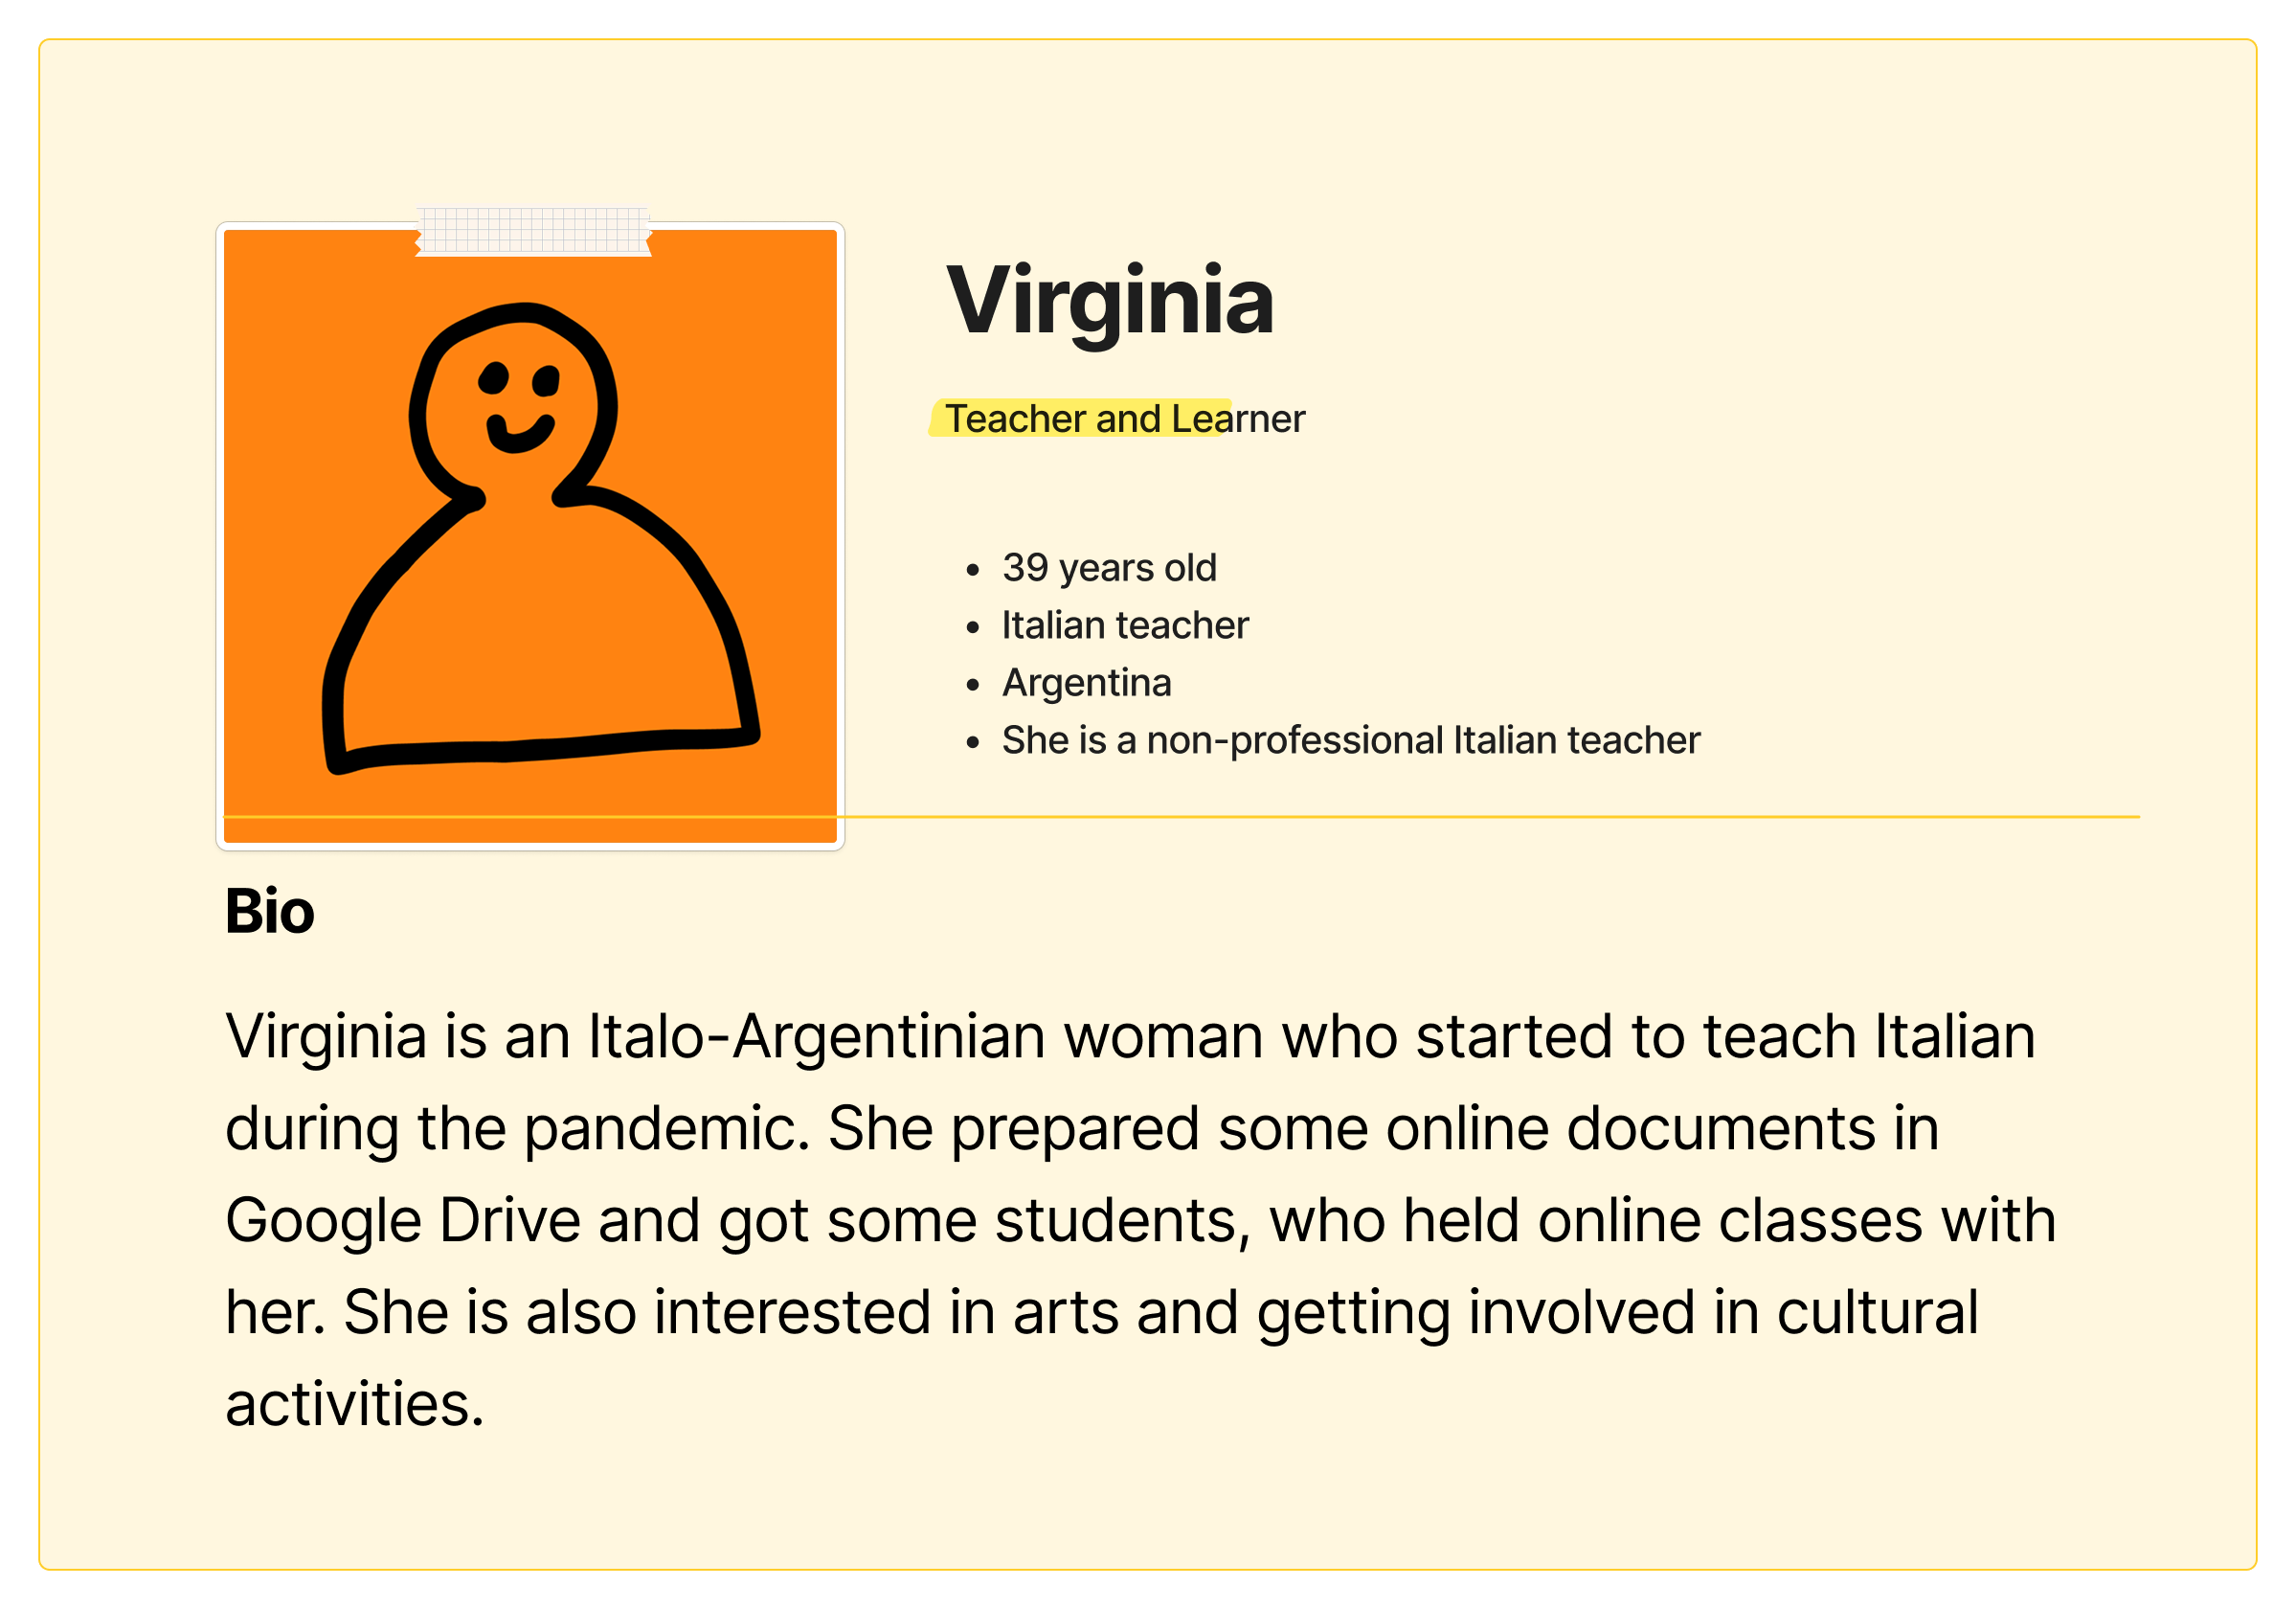
\includegraphics[width=10cm]{teacher-and-learner}
    \caption{A 30-year-old language teacher interested in both teaching and learning other things.}
    \label{fig:figure16}
\end{figure}
\begin{figure}[b]
    \centering
    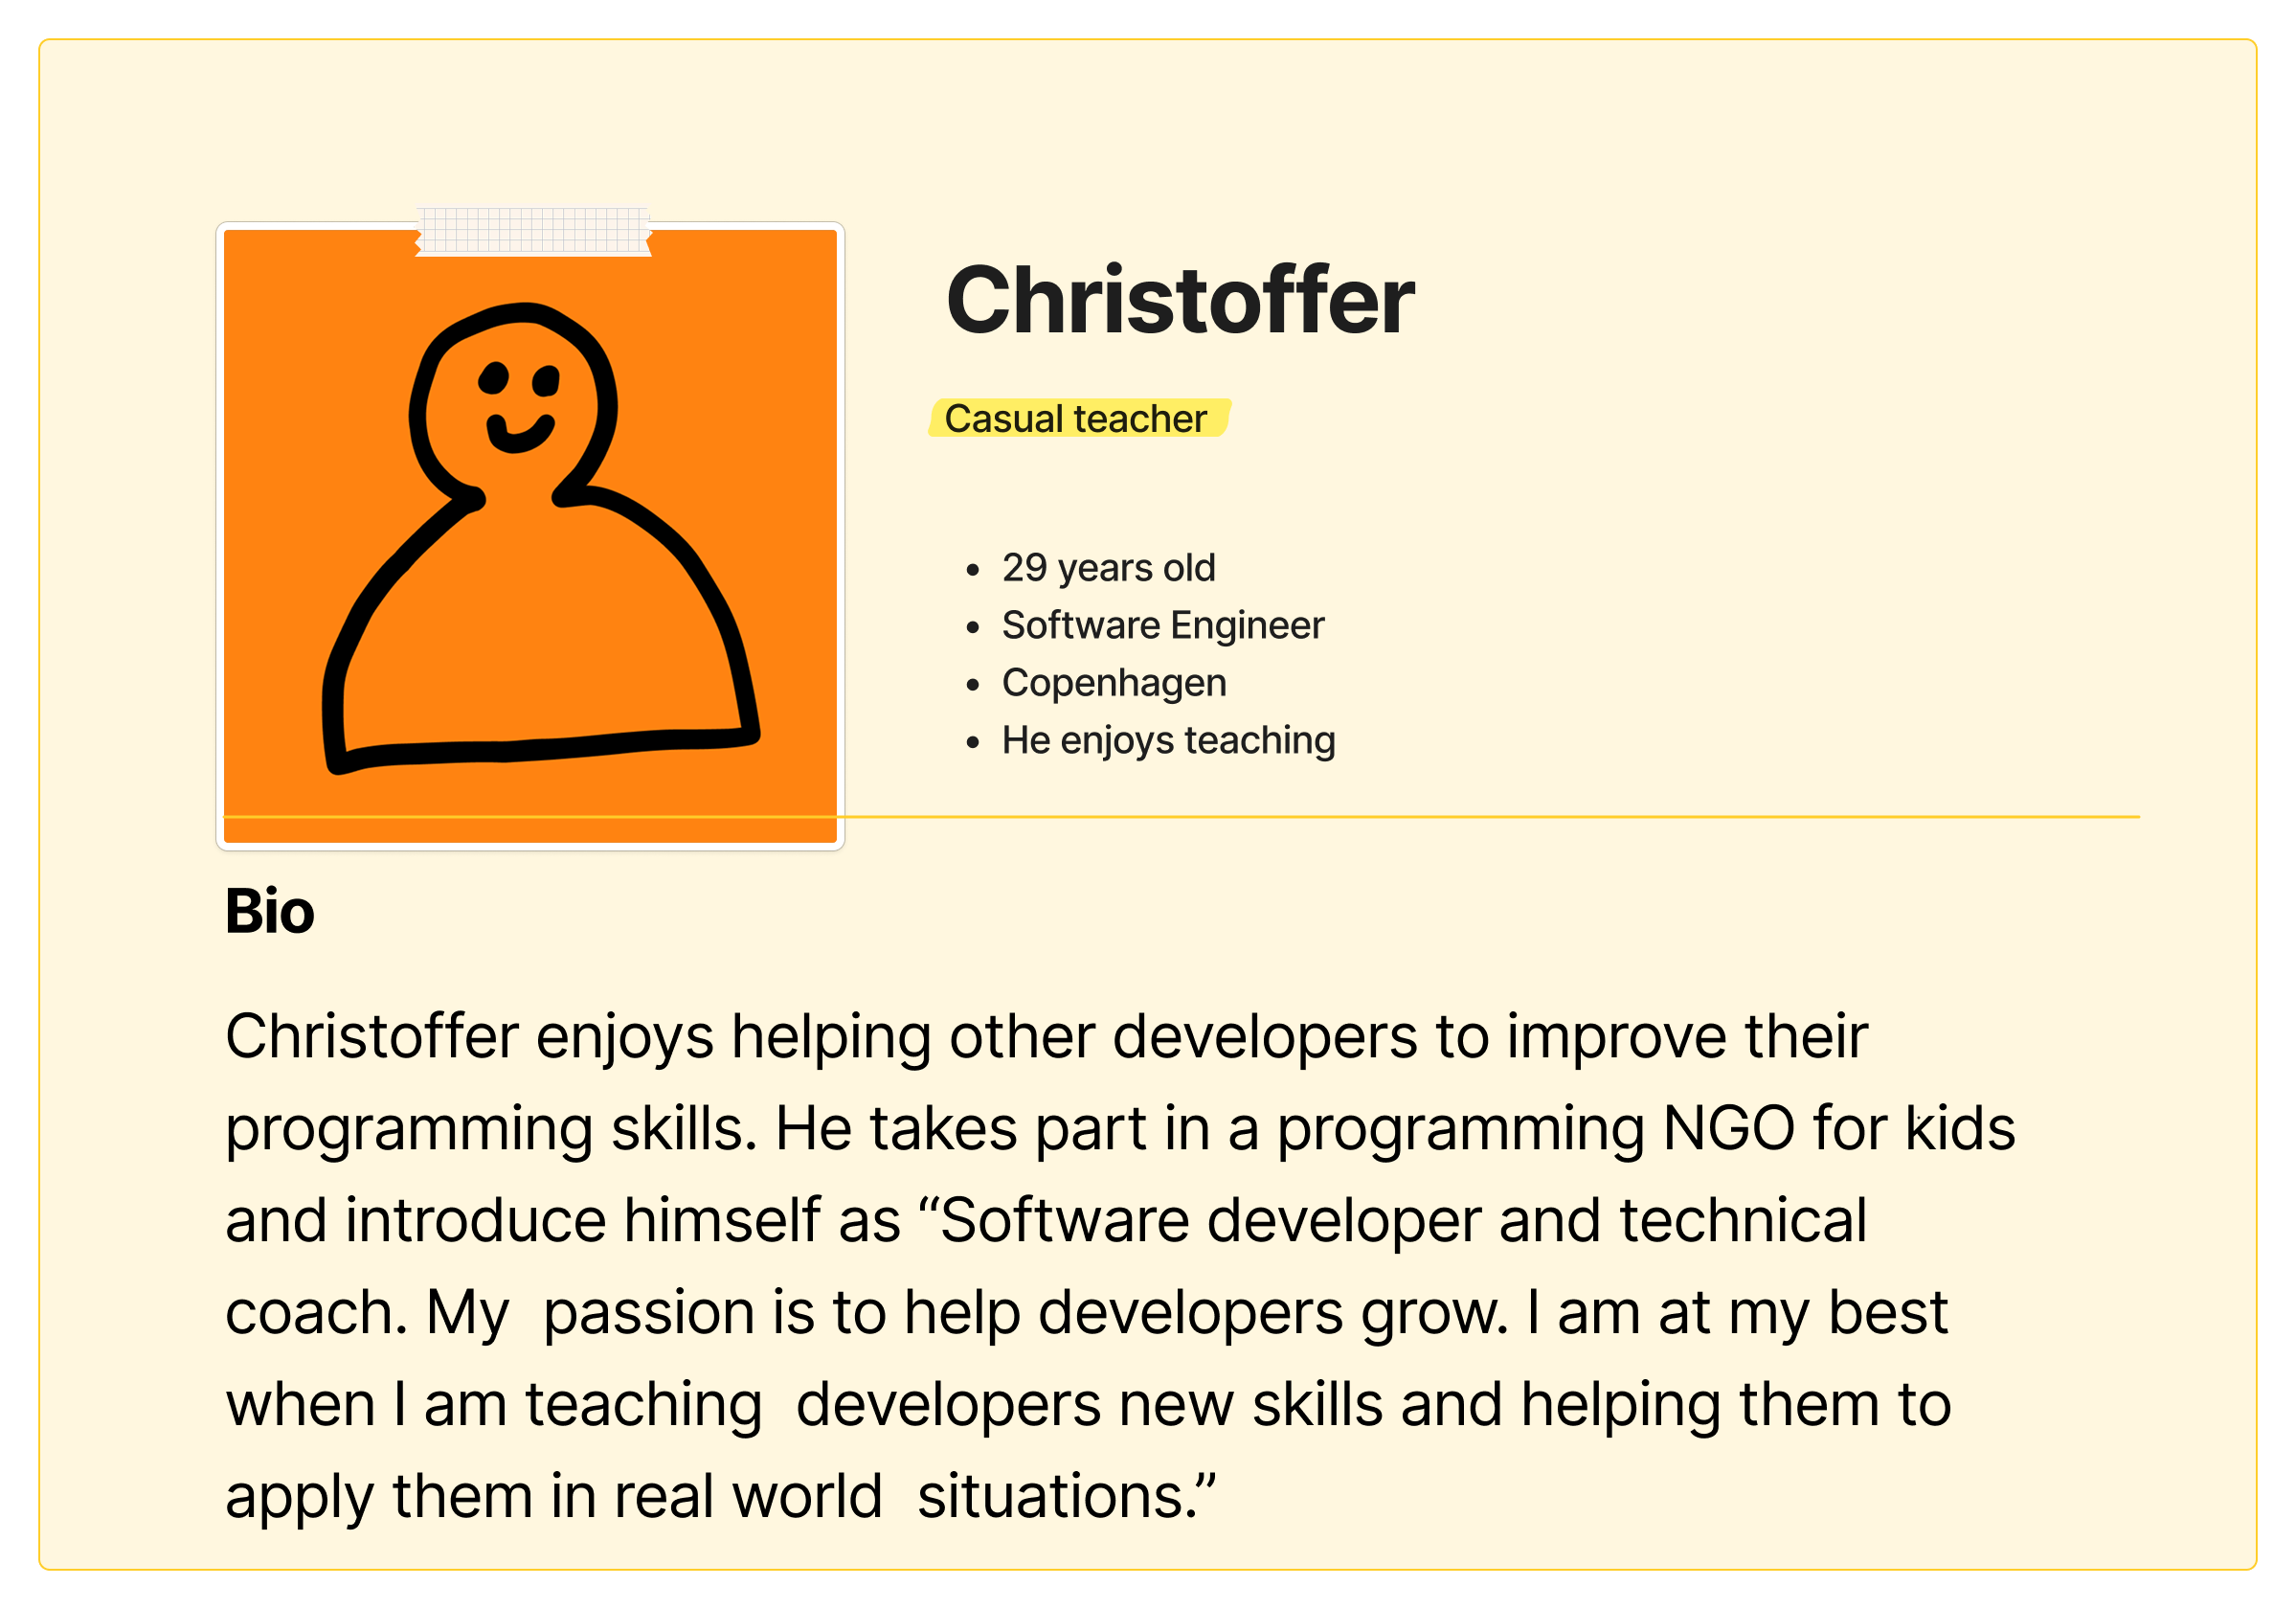
\includegraphics[width=10cm]{casual-teacher}
    \caption{ 29-year-old Software Engineer teaching for fun.}
    \label{fig:figure17}
\end{figure}

\clearpage

\subsubsection{User Flows}\label{subsubsec:user-flows}
As mentioned before, the team prioritized the user flows instead of user journey maps.
Often, these tools are used interchangeably, but they have different purposes.
In the ideation phase of UX design, user journeys and user flows are two essential tools, both structured around achieving user goals.
While they share the common objective of understanding and improving user experiences, they differ in scope and purpose.
A user journey represents the sequence of steps a user takes to accomplish a high-level goal.
This process is typically documented through journey maps, which visualize the user's path across different touch-points.
In contrast, a user flow focuses on a more granular objective within a single product, offering a detailed view of how users interact with specific features or tasks.
Artifacts associated with user flows include wireflows, flowcharts, and task diagrams, which outline the exact steps and decision points users encounter.\newline
User flows are particularly valuable because they promote user-centered design by clarifying what the product should do, the sequence in which tasks should be performed, and the information that must be presented at each stage.
This structured approach not only enhances the user experience but also accelerates development and reduces errors by providing a clear and logical framework for designers and developers to follow.\cite[User Journeys vs User Flows]{userJourneys}

During the ``discovery'' and ``define'' phases of the Double Diamond framework, the team realised that one of the most key user journeys on the platform, was the sig-up journey.
One of the the reason for this is that the sign-up process is the first interaction a user has with the platform, and it sets the tone for the rest of their experience.
But also, it is in this interaction that the user will provide the most important information about themselves, like their skills, their interests and what type of user they might be.

For us to understand how to design and develop this main part of the website, we did a high level sign-up user flow and a kind of ``internal'' user flow, within the sign-up process, to comprehend the different steps and decisions the user would have to make to complete the sign-up process.
These user flows were a good starting point to understand how we could gather all the necessary information from our users to create their profile and internally understand what type of user they are.
Also, it was a good way to cover all the different decisions the user would have to make to complete the sign-up journey.
\begin{figure}[h]
    \centering
    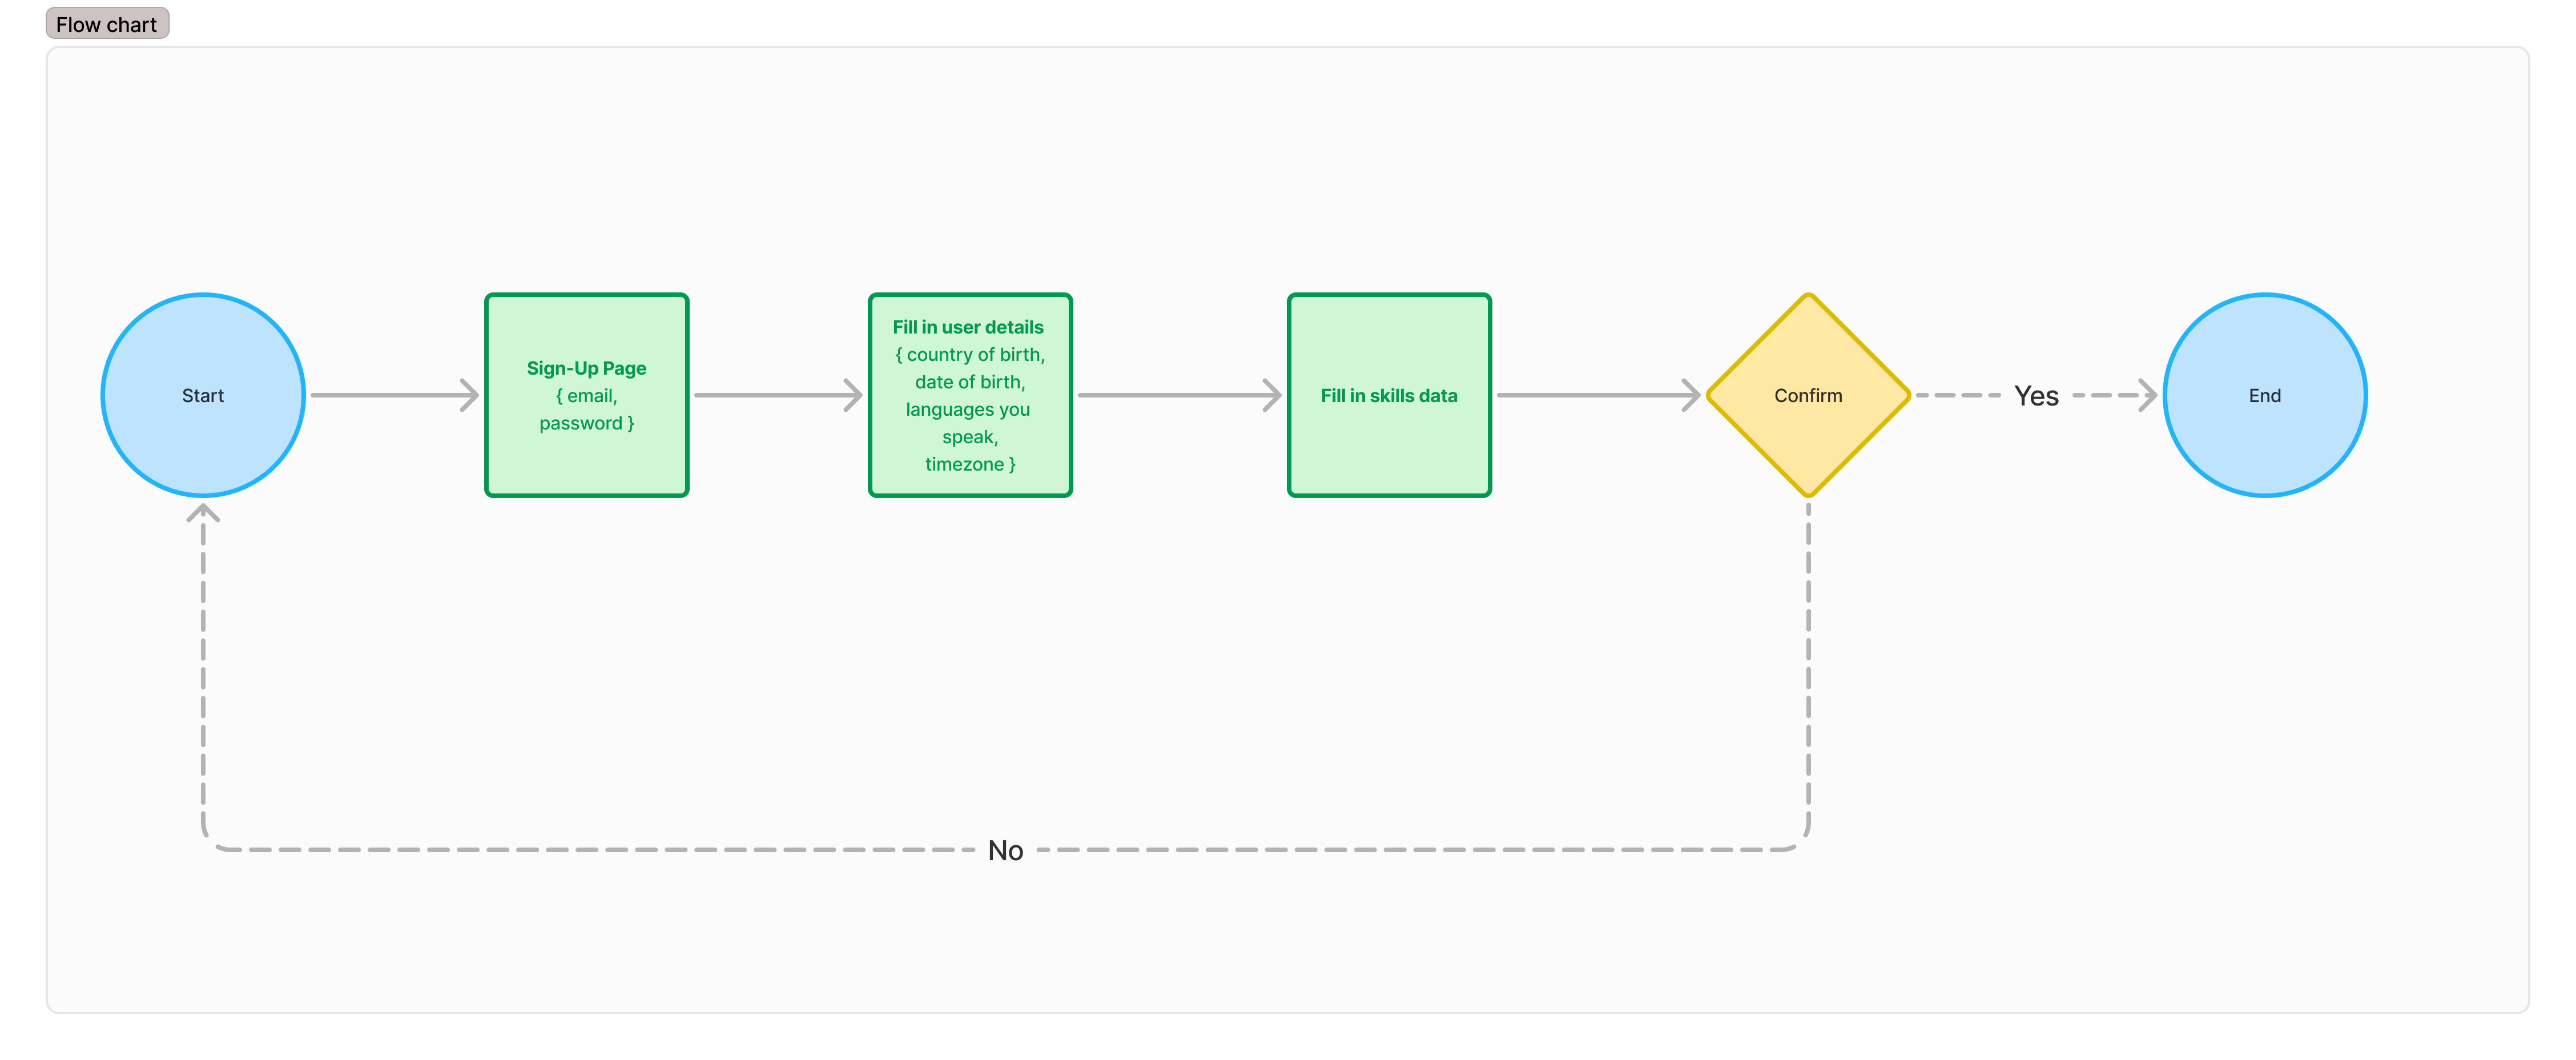
\includegraphics[width=15cm]{sign-up-flow}
    \caption{High level sign-up user flow.}
    \label{fig:figure18}
\end{figure}
\newpage
\begin{figure}[h]
    \centering
    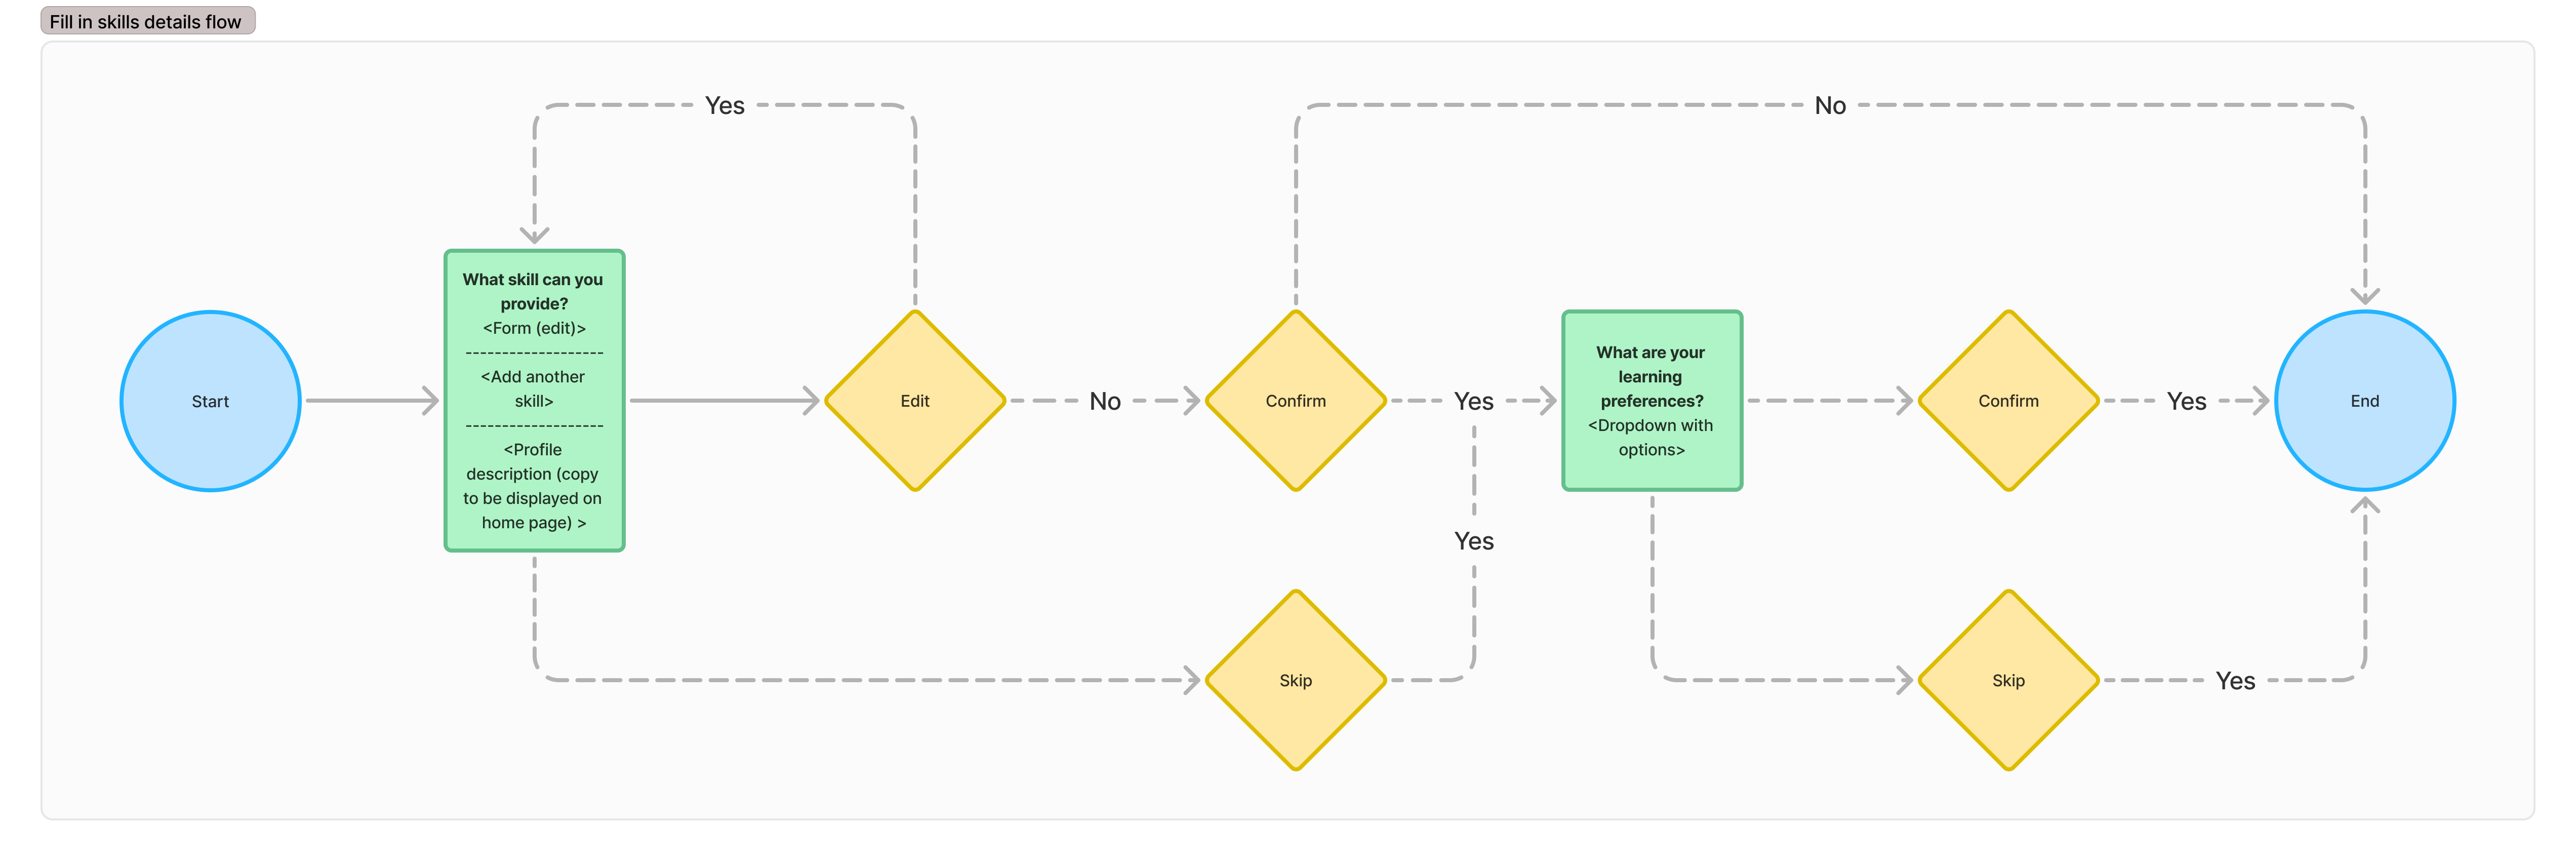
\includegraphics[width=15cm]{fill-in-skills-flow}
    \caption{Fill in skills user flow - within high level flow}
    \label{fig:figure19}
\end{figure}

\subsection{User Interface Design}\label{subsec:user-interface-design}
As with the user experience design, the development of Chronocademy’s User Interface (UI) was based on user research and competitive analysis.
The team aimed to create an intuitive and visually engaging interface that aligned with users’ needs while maintaining consistency with the platform’s core features.
Insights from user interviews and competitor analysis played a key role in shaping the interface, ensuring that the visual elements supported a seamless and efficient user experience.\newline
To structure the UI design process, the team prioritized clarity, usability, and aesthetic coherence, focusing on creating an interface that enhances navigation while reinforcing Chronocademy’s brand identity.
The MVP (Minimum Viable Product) methodology also guided the interface design, ensuring that essential features, such as the sign-up journey, communication channels between users, and user profiles, were clearly and effectively presented in the initial release.\newline
While time constraints limited the implementation of advanced design methods like high-fidelity prototypes and design systems, the team relied on wireframes, low-fidelity prototypes, and iterative feedback loops to refine the interface.
This approach allowed for continuous improvement, ensuring that the interface was both functional and aligned with user expectations.
The team believes that by maintaining a close connection between the UX research and UI design, the team was able to deliver an interface that not only meets user needs but also provides a cohesive and engaging platform experience.

\subsubsection{Reusable components}\label{subsubsec:rereusable-components}
To ensure consistency and efficiency in the UI design process, the team created a library of reusable components.
A reusable component can be defined as a self-contained element that can be used across different screens or pages of a digital product.
These components included buttons, icons, dropdowns, and other interface elements that could be easily replicated across different screens.
By standardizing these components, the team ensured a cohesive and visually appealing design while streamlining the development process.
Here are some examples of reusable components created for Chronocademy's UI design and more can be found in the appendix.

\begin{figure}[h]
    \centering
    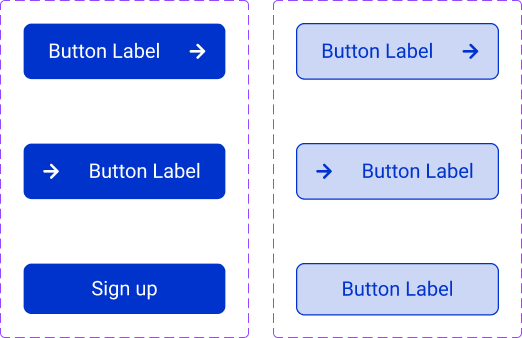
\includegraphics[width=5cm]{reusable-buttons}
    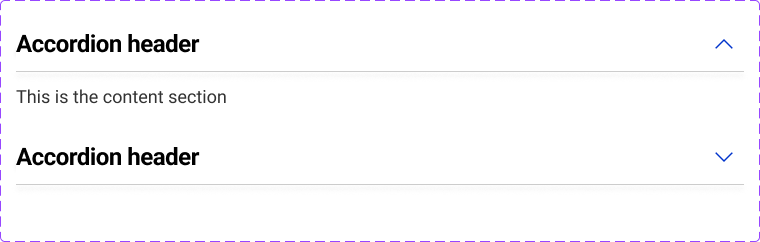
\includegraphics[width=5cm]{reusable-accordeon}
    \caption{Reusable components for Chronocademy's UI design.}
    \label{fig:figure20}
\end{figure}

\subsubsection{Brand guidelines}\label{subsubsec:brand-guidelines}
In addition to reusable components, the team developed brand guidelines to ensure consistency in the platform's visual identity.
\newpage
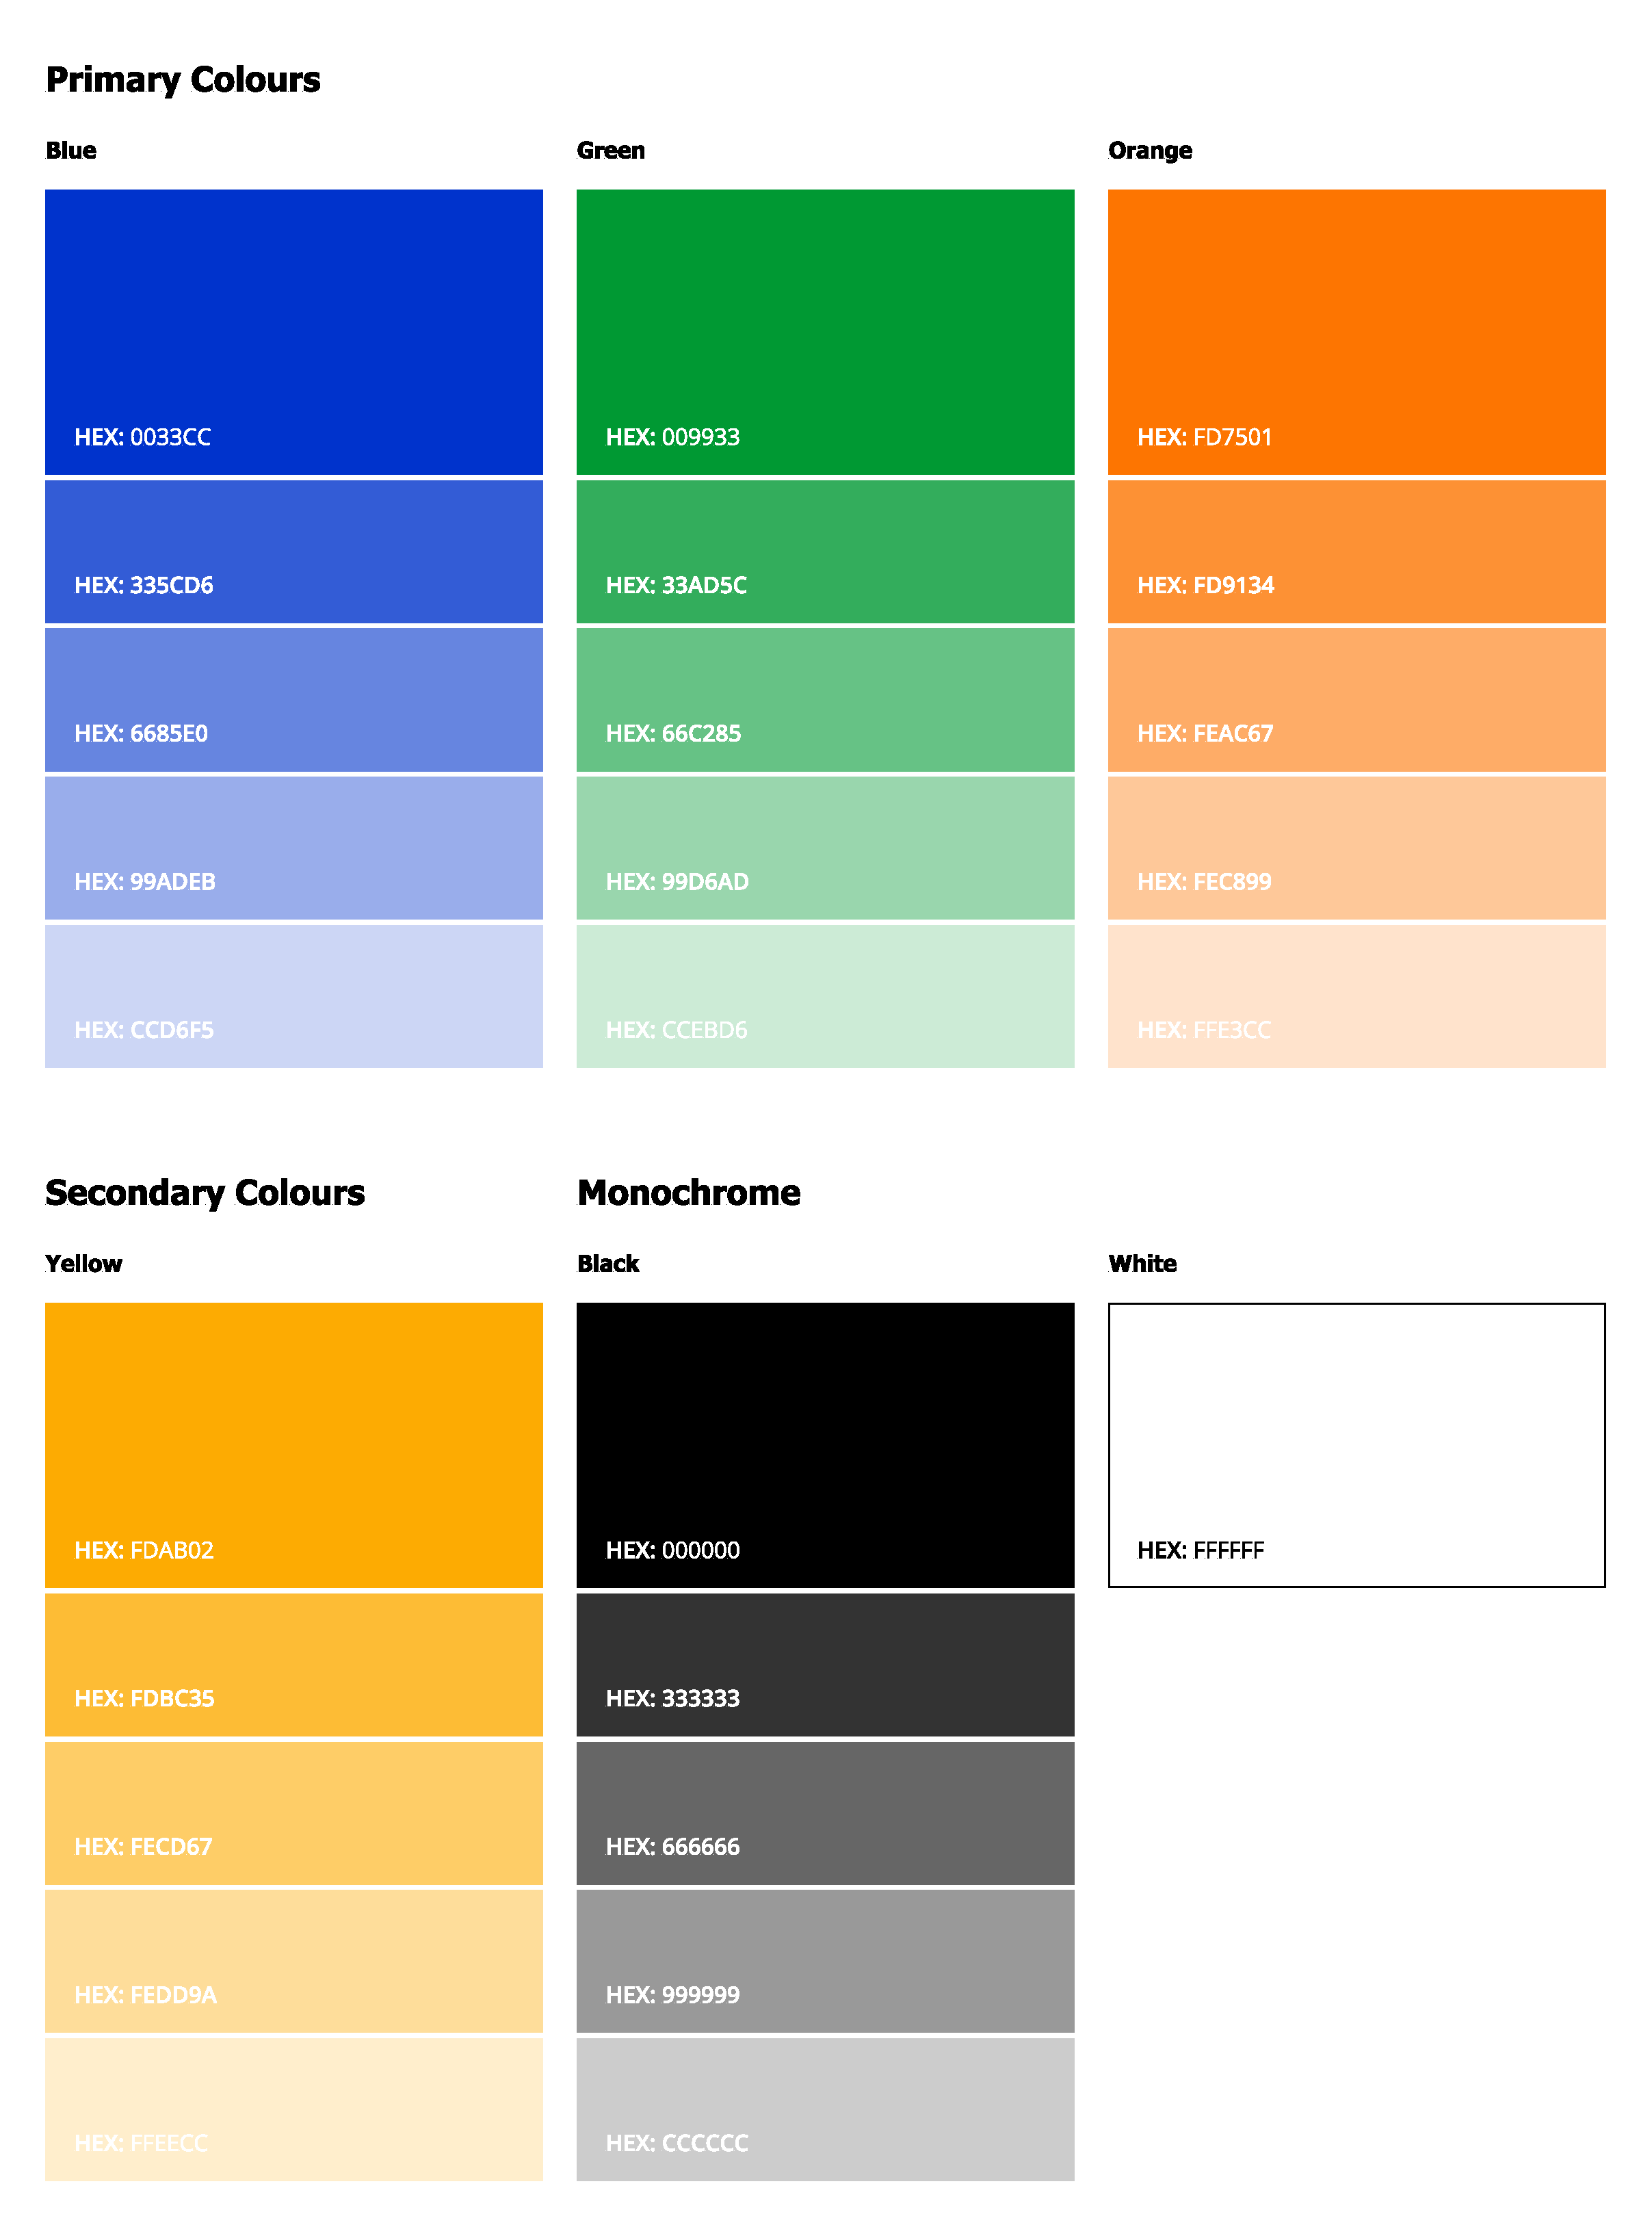
\includepdf[pages=-]{brand-colors.pdf}
\newpage
\subsubsection{Wireframes}\label{subsubsec:wireframes}
Wireframes are low-fidelity visual representations of a digital product's layout and structure.
They are ``essentially a blueprint of your app.
A basic 2D outline that gives you an idea of the elements and features that will appear in the final app.''\cite[Wireframes]{lowFidelity}
The team used this design tool to quickly sketch the layout of the platform, focusing on the placement of key elements and the overall user flow and get some fast feedback from the team and potential users.\newline\newline
The sign-up journey wireframe was initially built with pencil and paper, to understand the different steps and decisions the user would have to make to complete the sign-up process and how to represent this visually.
While other wireframes (other parts of the application), were directly built digitally, using a design software.
The wireframe covered ``areas'' of the app were:
\begin{enumerate}
    \item Sign-up
    \item Sign-in / Sign-out
    \item Home page
    \item User profile
    \item Public profile / Communication channel
\end{enumerate}
For brevity, we will only show the some wireframes, but the other wireframes can be found in the appendix.\newline
\begin{figure}[h]
    \centering
    \rotatebox{90}{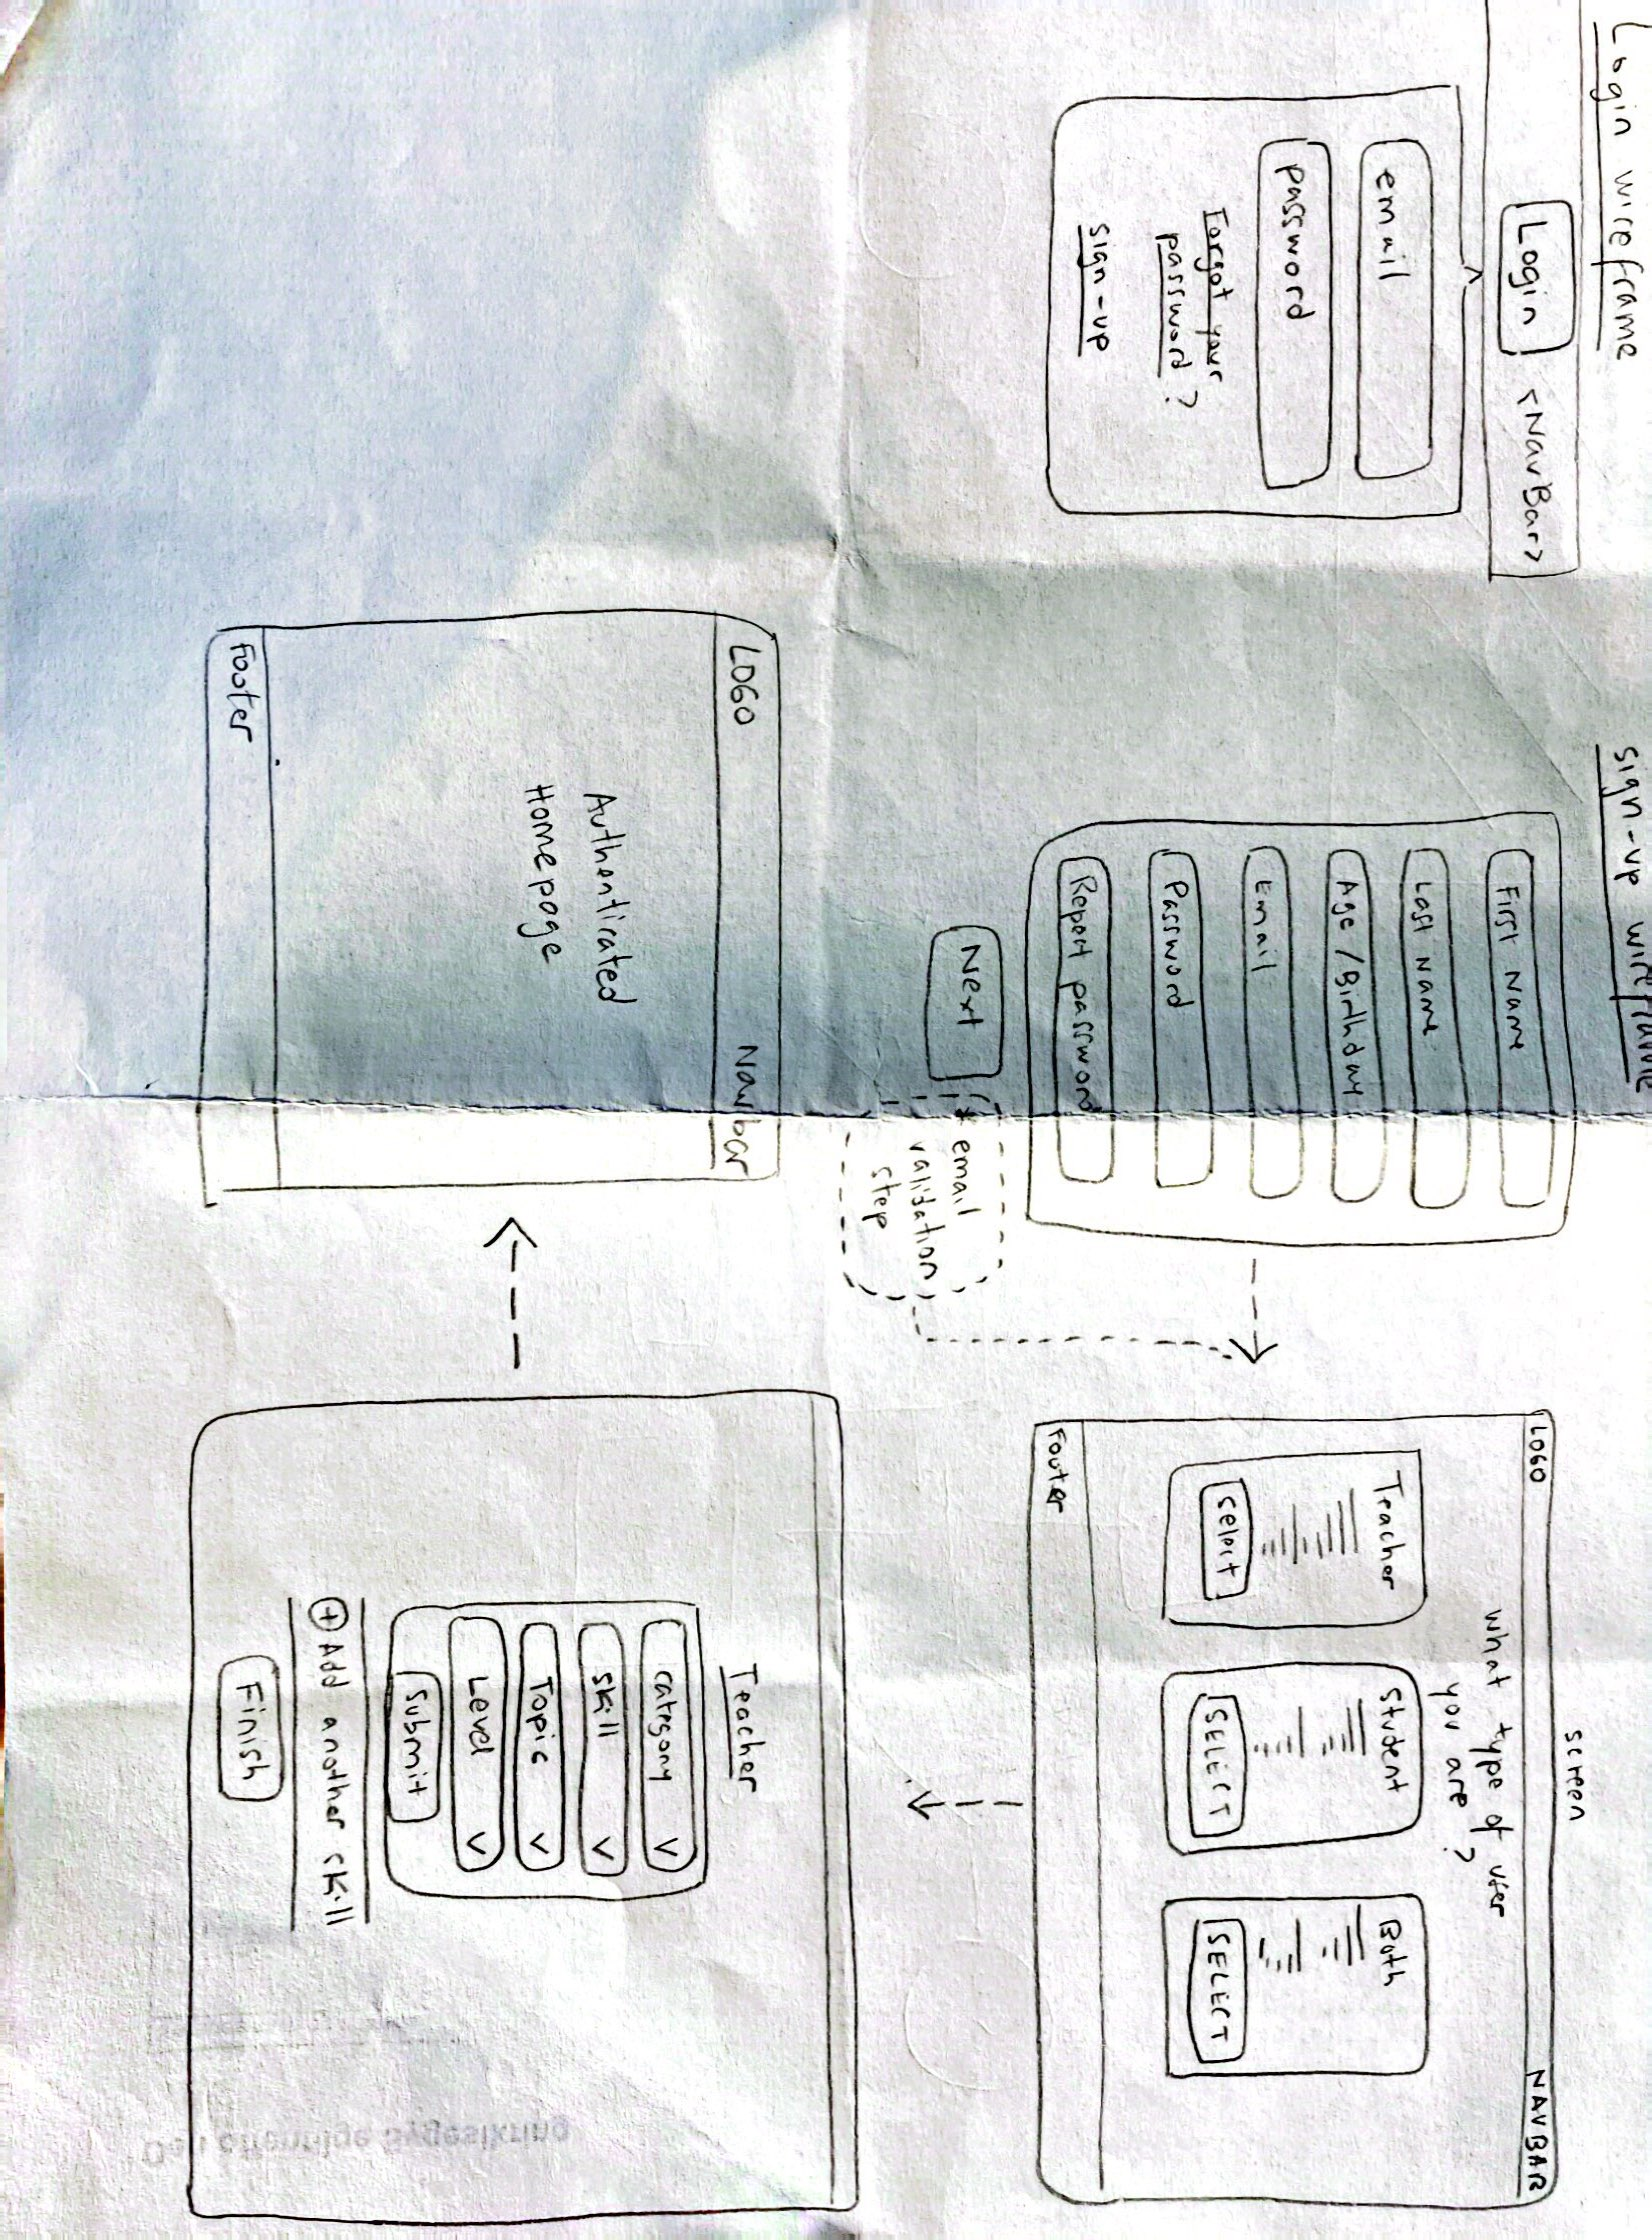
\includegraphics[width=10cm]{wireframe-authentication}}
    \caption{Authentication wireframe.}
    \label{fig:figure21}
\end{figure}
This wireframe shows the initial user authentication journey for Chronocademy, guiding users through key stages such as login, sign-up, profile selection, and skill input.
The process begins with the Login Page, where users can access their accounts by entering their email and password.
This page also includes options to retrieve a forgotten password and a link for new users to sign up.
For those who choose to Sign Up, the next step involves providing important details such as first name, last name, among others.
Following the sign-up process, users arrive at the Profile Type Selection screen, where they define their role on the platform.
They can choose to register as a Teacher, Student, or Both.
If the user selects the Teacher role (or both), they are directed to a Skill Input page.
Here, they can specify their areas of expertise through dropdown fields for skill, category, topic, and proficiency level.
The option to Add Another Skill allows users to input multiple competencies, and a Submit button finalizes their entries.
Once this information is complete, the user clicks Finish to access the homepage view.
This page includes a logo for brand identity, a navigation bar (navbar) for easy access to core features, and a footer providing additional resources or links.
Although the first iteration of the wireframe laid the foundation for this journey, the final design evolved in a different direction based on further insights and refinements.
Nonetheless, this initial wireframe was invaluable in shaping the platform's structure and provided a solid basis for future design decisions.\newline\newline

\begin{figure}[h]
    \centering
    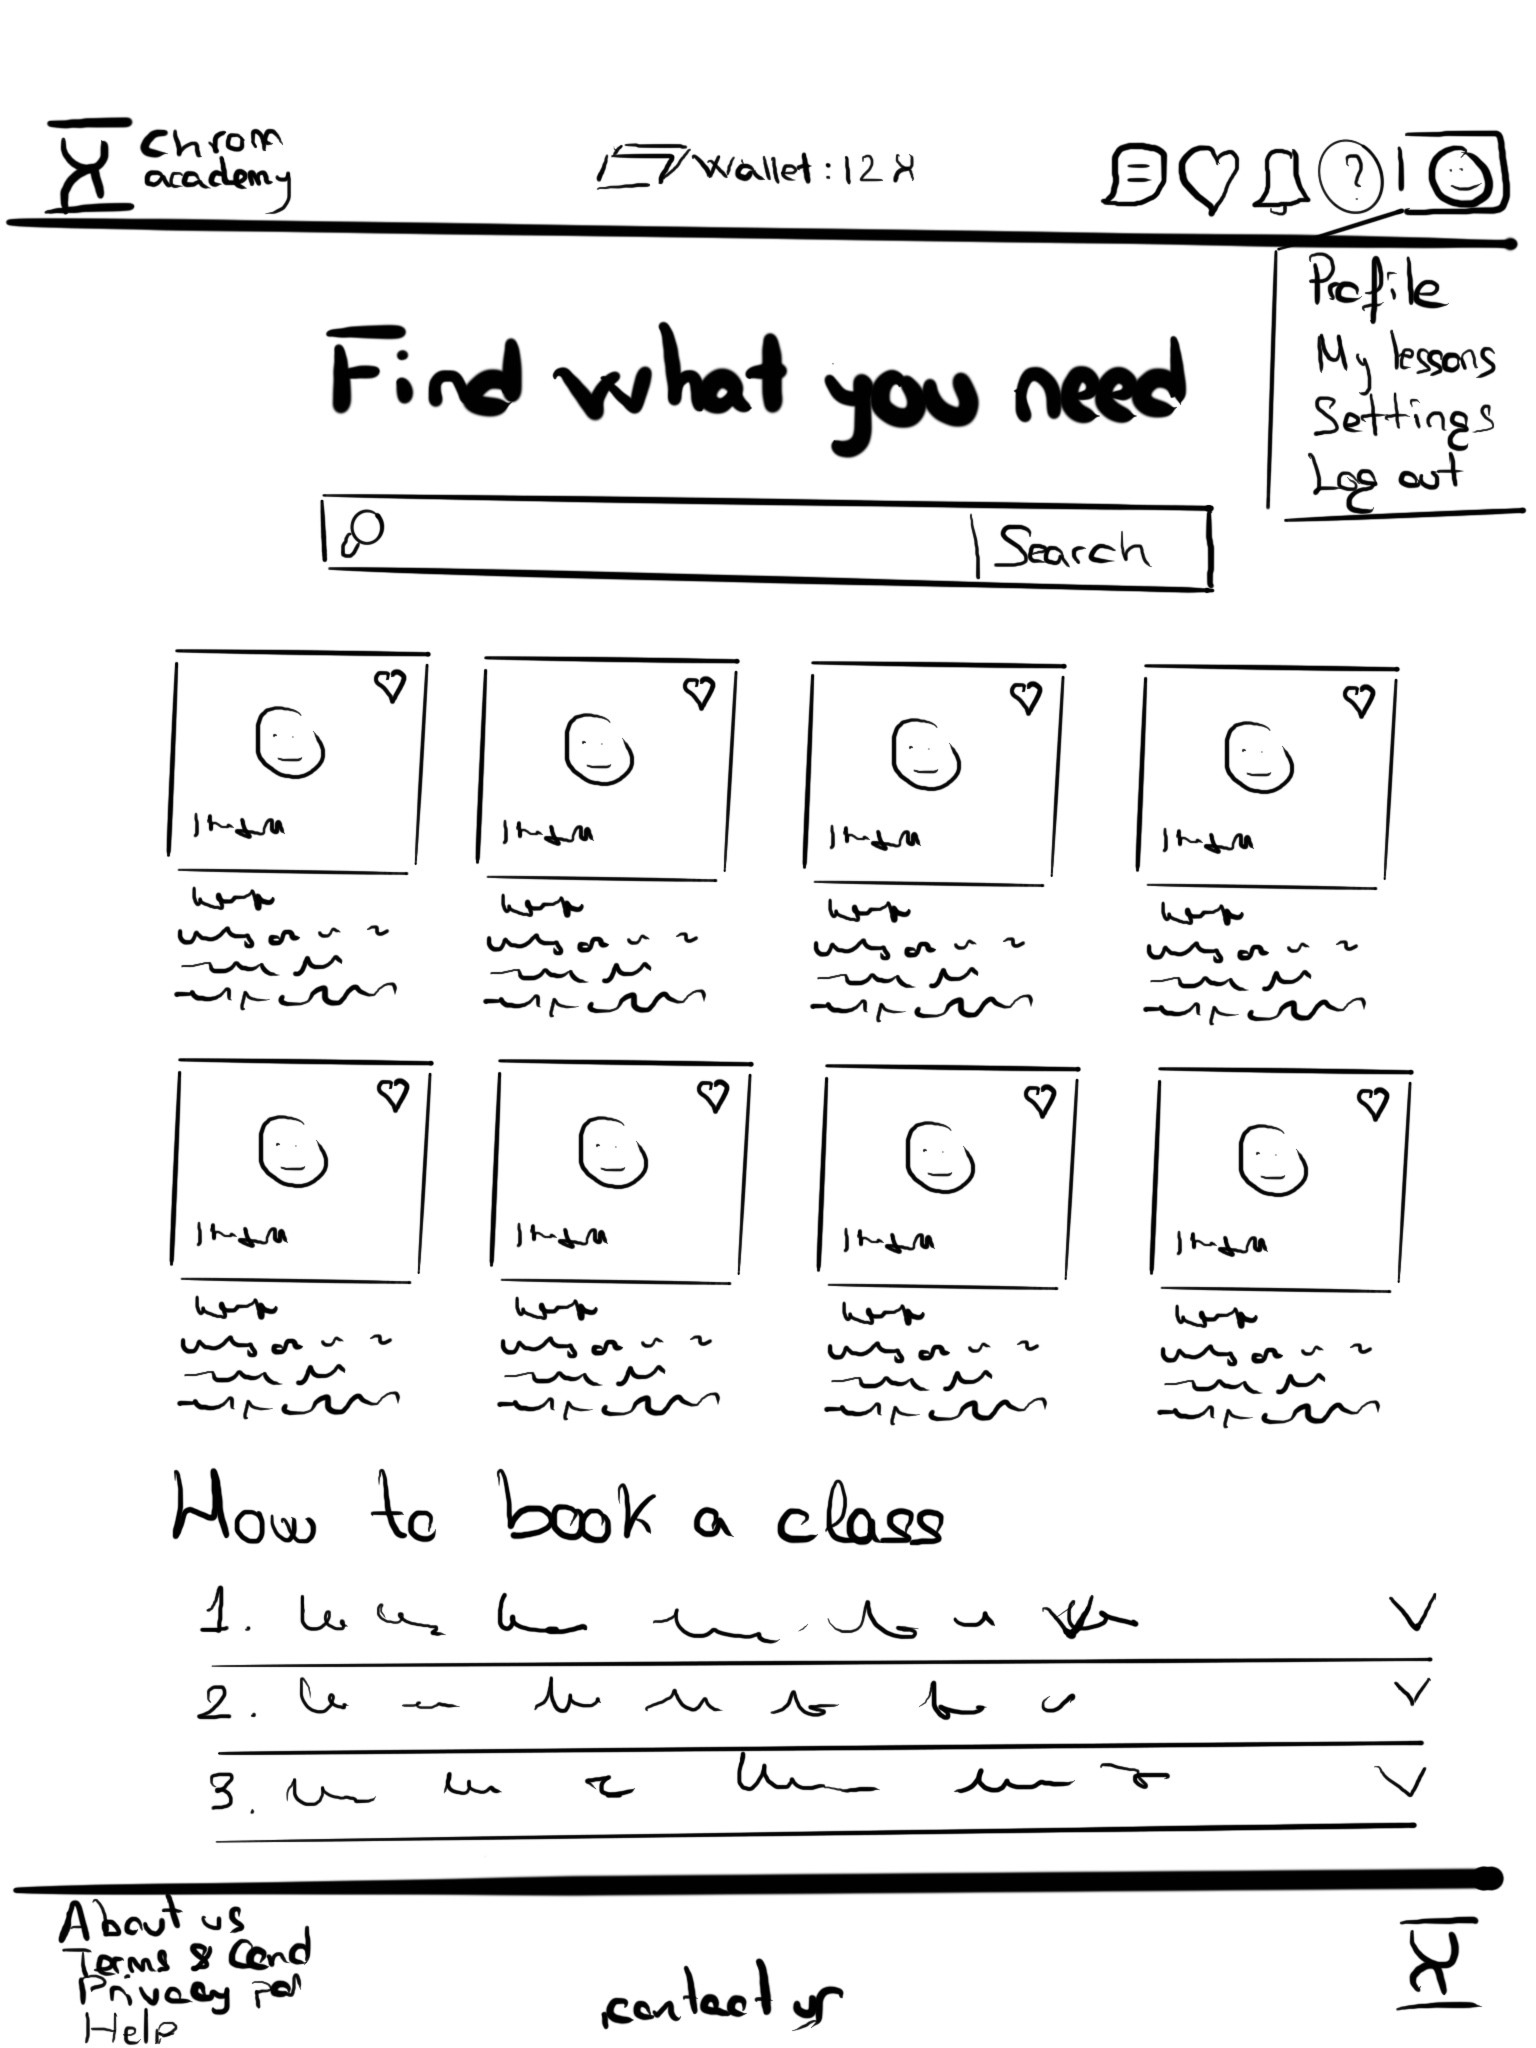
\includegraphics[width=10cm]{wireframe-home-page}
    \caption{Home page wireframe.}
    \label{fig:figure22}
\end{figure}
This wireframe represents the home page of Chronocademy, designed to help users quickly find and book lessons.
At the top, there’s a header with the Chronocademy logo on the left and a wallet indicator showing the user's balance.
On the right, there are several icons for key features like chat, notifications, help, and a profile menu where users can access their profile, lessons, settings, or log out.
The main section features a search bar under the title ``Find what you need'', allowing users to look for classes or instructors.
Below the search bar is a grid of instructor profiles, each showing a profile picture, name, and a brief description.
Users can also favorite instructors by clicking the heart icon on each card.
Further down, there’s a ``How to book a class'' section that outlines the steps for scheduling lessons.
Each step is collapsible, making it easy for users to expand and get more details if needed.
At the bottom, the footer provides links to About Us, Terms \& Conditions, Privacy Policy, Help, and a Contact Us option.
Unlike the previous wireframe, this one was created digitally, allowing for more detailed design elements and it did not change significantly in the final design.\newline
\indent The team found wireframing to be the most convenient and effective design tool throughout the Chronocademy project.
Compared to high-fidelity prototypes, wireframes are much easier and faster to create, as they do not require advanced design skills or specialized software knowledge.
This made the process more accessible to the entire team, allowing everyone to contribute ideas visually.
Wireframes also enabled us to quickly sketch out concepts, gather feedback, and iterate on designs without spending too much time on polished visuals.
This approach helped us refine our ideas efficiently and laid a strong foundation for the platform’s development.

\subsubsection{Prototypes}\label{subsubsec:prototypes}
As mentioned before, the team did not have the time to create high-fidelity prototypes, but the wireframes were a good starting point to understand the different steps and decisions the user would have to make and how to represent this visually.
But the team did create some kind of low-fidelity prototypes to test the platform with real users and gather feedback.
We say ``kind of'' because what we prototyped it is actually a ``high fidelity'' prototype, but it is for the website landing page, so there were not that many features or interactions to implement.

By definition, a ux prototype is:
\begin{quote}
    ``a simulation or sample version of a final product, which is used for
    testing prior to launch.
    The goal of a prototype is to test products (or
    product ideas) before spending lots of time and money into the final
    product.''\cite[UX Deliverables]{uxDeliverables}
\end{quote}

Unlike the wireframes, the prototypes, require more time and effort to create.
And since the landing page is the first interaction a user has with the platform, the team decided to create a high-fidelity prototype to get it right.
The reason behind this, is that the latter type, involves much more detail and often includes design elements like colors, images, and typography.
A recognised design agency, Decode, explains that:
\begin{quote}
    ``While a low-fidelity wireframe deals with broader strokes, a high-fidelity wireframe is concerned with more granular details.
This can include layout, information architecture, and spacing.
In some cases, a high-fidelity wireframe achieves a level of detail that makes it look like the final version of the app.
This is called a mockup, a planning tool used to illustrate the final UI design of the app.
High-fidelity wireframes could include interactive elements like clickable links or buttons.
At this point, such a wireframe becomes a prototype, which is used to test the usability of an app with end users.''\cite[Low-fidelity vs High-fidelity]{lowFidelity}
\end{quote}

All in all, prototyping—alongside wireframing—played a crucial role in shaping Chronocademy’s user experience and interface.
While wireframes allowed us to quickly sketch out ideas, gather feedback, and iterate efficiently without requiring advanced design skills, prototypes gave us a more refined and interactive way to test key elements of the platform.

Although time constraints prevented us from creating high-fidelity prototypes for every feature, developing a high-fidelity landing page prototype was a strategic decision.
As the landing page is a user's first interaction with the platform, investing time and effort into a polished prototype helped us ensure a clear, engaging, and user-friendly experience.

Throughout the UX/UI process, we found that low-fidelity tools like wireframes were the most practical for rapid ideation and iteration.
However, high-fidelity prototypes proved valuable when precision and visual clarity were necessary—especially for user-facing components like the landing page.
This balanced approach allowed us to combine speed and flexibility with attention to detail, enabling the team to refine both the user journey and the interface design effectively.

Overall, our UX/UI process combined structured methodologies like the Double Diamond and user flows with hands-on design tools like wireframes and prototypes.
This iterative approach not only helped us understand user needs and behaviors but also allowed us to continuously improve our designs based on real user feedback.
By prioritizing accessible and adaptable design practices, we were able to develop a platform that aligns with both user expectations and the project’s core objectives.

In the next page, the reader can find the high-fidelity prototype for the landing page of Chronocademy.
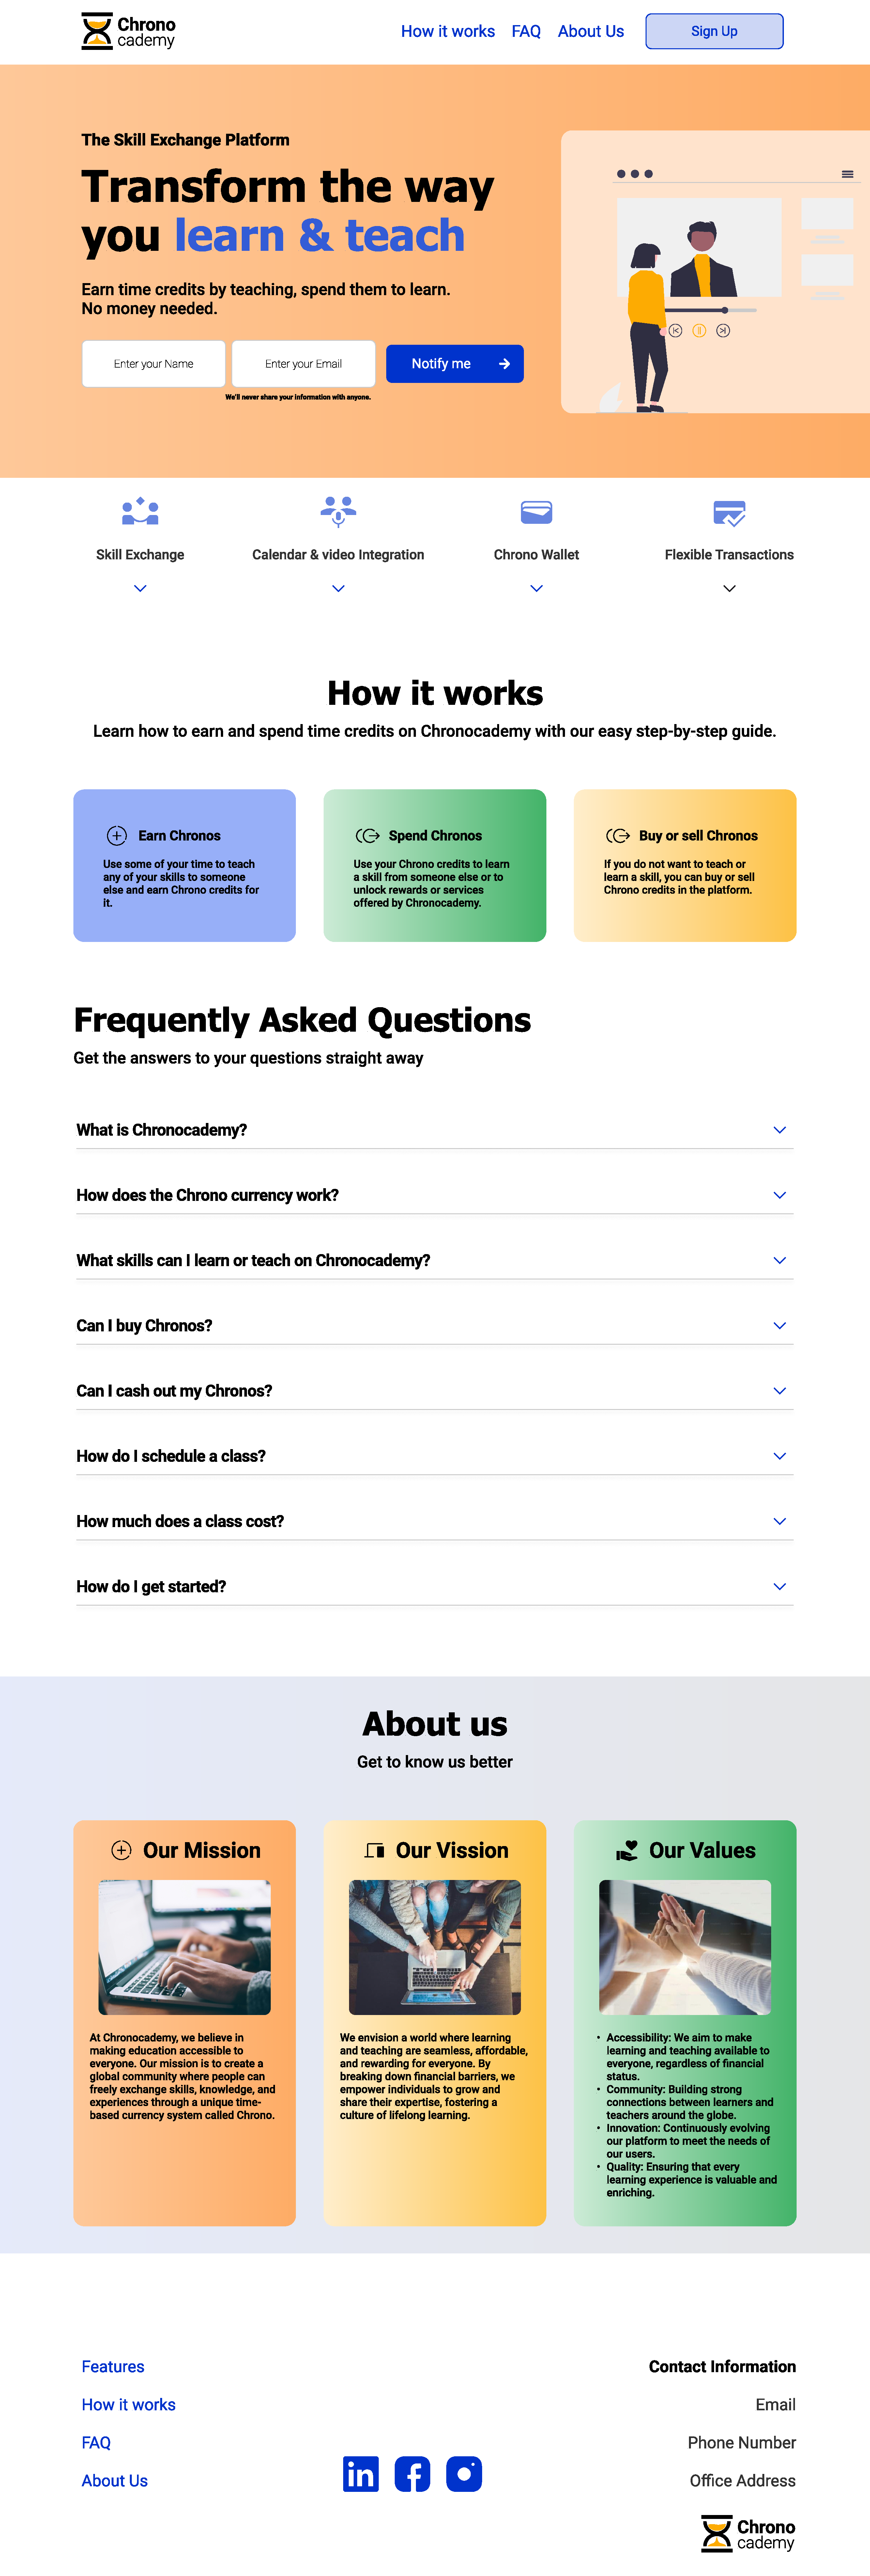
\includepdf[pages=-]{prototype-landing-page.pdf}